\documentclass[11pt,a4paper]{article}
\usepackage[T1]{fontenc}
\usepackage{iftex}
\ifPDFTeX\usepackage[utf8]{inputenc}\fi
\usepackage{lmodern}
\usepackage[a4paper,margin=21mm,headheight=15pt]{geometry}
\usepackage{microtype,graphicx,xcolor,booktabs,tabularx,array,enumitem,fancyhdr}
\usepackage{tikz}
\usetikzlibrary{arrows.meta,positioning}
\usepackage{tcolorbox}
\usepackage{xurl,hyperref,titlesec}
\usepackage[font=small,labelfont=bf,justification=raggedright,singlelinecheck=false]{caption}
\definecolor{navy}{HTML}{142B45}
\definecolor{teal}{HTML}{147A78}
\definecolor{pale}{HTML}{EEF5F5}
\definecolor{muted}{HTML}{596878}
\hypersetup{colorlinks=true,linkcolor=navy,urlcolor=teal,pdftitle={Continuum: Project and Quality Audit Report},pdfauthor={Ayush / Codex},pdfsubject={Architecture, verification and 120 actionable quality findings}}
\titleformat{\section}{\Large\bfseries\color{navy}}{\thesection}{.6em}{}
\titleformat{\subsection}{\large\bfseries\color{navy}}{\thesubsection}{.6em}{}
\titlespacing*{\section}{0pt}{12pt}{8pt}
\titlespacing*{\subsection}{0pt}{10pt}{5pt}
\setlength{\parindent}{0pt}
\setlength{\parskip}{6pt}
\setlength{\emergencystretch}{2em}
\setlist[itemize]{leftmargin=1.3em,itemsep=3pt,topsep=4pt}
\setlist[enumerate]{leftmargin=1.5em,itemsep=3pt,topsep=4pt}
\renewcommand{\arraystretch}{1.16}
\renewcommand{\tabularxcolumn}[1]{>{\raggedright\arraybackslash}p{#1}}
\newcolumntype{P}[1]{>{\raggedright\arraybackslash}p{#1}}
\pagestyle{fancy}\fancyhf{}
\fancyhead[L]{\small\color{muted}CONTINUUM / PROJECT QUALITY}
\fancyhead[R]{\small\color{muted}23 OCTOBER 2026}
\fancyfoot[L]{\small\color{muted}Baseline \texttt{1ec26fb0b59c}}
\fancyfoot[R]{\small\thepage}
\renewcommand{\headrulewidth}{.3pt}
\newtcolorbox{note}{colback=pale,colframe=teal,boxrule=.4pt,arc=1.5mm,left=3mm,right=3mm,top=2mm,bottom=2mm}
\newenvironment{finding}[3]{\par\vspace{3pt}\begin{minipage}{\textwidth}\hypertarget{#1}{}%
{\color{teal}\rule{\textwidth}{.6pt}}\par\vspace{2pt}%
{\small\bfseries\color{teal}#1\quad #2}\par\vspace{1pt}%
{\large\bfseries\color{navy}#3}\par\vspace{2pt}%
\small\setlength{\parskip}{4pt}}{\end{minipage}\par\vspace{7pt}}
\DeclareRobustCommand{\issue}[1]{\hyperlink{#1}{\texttt{#1}}}
\newcommand{\src}[1]{{\small\path{#1}}}
\begin{document}\hypersetup{pageanchor=false}
\begin{titlepage}\thispagestyle{empty}
{\small\bfseries\color{teal}ENGINEERING PROJECT REPORT}\par
\vspace{20mm}
{\fontsize{40}{44}\selectfont\bfseries\color{navy}Continuum}\par
\vspace{4mm}
{\LARGE\color{navy}Assessment continuity,\par collaboration and recovery}\par
\vspace{12mm}
{\Large Project analysis and quality audit}\par
{\large Architecture, verification, risks and a prioritized fix backlog}\par
\vspace{14mm}
\begin{note}
{\fontsize{30}{34}\selectfont\bfseries\color{teal}120}\quad actionable findings\par
68 defects, with additional hardening, policy, accessibility,\par performance, documentation and polish work clearly labeled.
\end{note}\vfill
\begin{tabularx}{\textwidth}{@{}lX@{}}
Project & Continuum, in the Slate repository \\
Repository maintainer & Ayush \\
Analysis and preparation & Codex, with repository and local execution evidence \\
Review date & 23 October 2026 (Asia/Kolkata) \\
Source baseline & \texttt{1ec26fb0b59cb4704ccce28b93fc4046da5a35f4} \\
Scope & Go API, React frontend, memory/DynamoDB stores, boards, local recovery demo and supported AWS configuration \\
\end{tabularx}\vspace{8mm}
{\small\color{muted}Engineering audit edition. Source-reviewed risks and product decisions are distinguished from reproduced defects.}
\end{titlepage}
\pagenumbering{roman}\hypersetup{pageanchor=true}

\section*{Abstract}\addcontentsline{toc}{section}{Abstract}
Continuum combines timed academic assessments with classroom coordination and a recovery demonstration. Its Go backend implements authentication, teacher authoring, learner attempts, grading, replayable submission receipts, membership and collaborative boards. A React frontend exposes the learner and teacher workflows. The supported cloud design uses two application instances across Availability Zones in one selected AWS Region, a regional DynamoDB table, an API Gateway/Lambda routing layer and a monitored Step Functions recovery workflow.

The implementation contains meaningful safeguards: immutable final submission request identities, transactional writer fencing, optimistic attempt versions, incident leases, readiness verification and audit reconciliation. Local execution confirmed the real-HTTP integration package, all eight browser journeys, all 167 frontend unit tests, type checking, linting, the frontend production build and Go vet. The complete race-enabled Go test command failed because two authentication tests use a fixed historical service clock while related validation still uses current time.

The review identifies 120 distinct actionable items. Of these, 68 are labeled defects; the remainder are explicitly classified improvements, hardening risks, policy gaps, accessibility issues or missing capabilities. Sixteen findings have isolated in-memory API probe evidence, one has direct browser observation and one has existing test-failure evidence. The remaining 102 are source-reviewed findings with a concrete trigger and acceptance criterion. These evidence labels describe verification depth; they do not claim that every item was reproduced in a browser or on AWS.

\begin{note}\textbf{Recommended focus.} Fix assessment start/deadline integrity, loss-prone learner autosave, board route/response contracts, concurrent authoring writes and mobile access to essential controls first. Resolve classroom privacy and review-release policies explicitly before applying the associated authorization changes.\end{note}
\textbf{Priority distribution:} 45 P1, 67 P2 and 8 P3. P1 means early attention because of integrity, access control, work-loss potential or a blocked core workflow. It is an engineering triage priority, not a security vulnerability score. No emergency P0 issue is asserted.
\clearpage\tableofcontents\clearpage\pagenumbering{arabic}

\section{Project purpose and current implementation}
\subsection{Problem and objectives}
Timed assessments depend on more than process availability. A healthy HTTP listener can still be unable to read questions or commit answers. A successful database write can also be followed by a lost response, leaving a learner unsure whether submission succeeded. Continuum addresses these conditions by retaining the learner's attempt timeline, identifying the final answer snapshot and recovering a matching receipt after disruption.

The broader product connects delivery with teacher authoring, classes, invitation codes, question reuse, results and live drawing. These workflows share services but do not all have the same resilience guarantees. Boards are outside the bounded HTTP assessment failover claim in the project documentation.
\subsection{Actors and implemented workflows}
\begin{tabularx}{\textwidth}{@{}P{26mm}X@{}}\toprule Actor & Current capabilities \\\midrule
Learner & Register/sign in, join classes, discover assigned exams, begin/resume a timed attempt, save partial answers, flag questions, submit, recover a matching receipt and review results. \\
Teacher & Create/edit classes, manage members/invitations, author and duplicate quizzes, import questions, maintain a bank, publish and change assessment settings, inspect results and control student drawing. \\
Operator & Inspect backend capability and epochs, inject bounded demonstration faults, verify recovery, request failback, reconcile work and pause/resume deployment through scripts. \\\bottomrule\end{tabularx}
\subsection{Functional coverage}
The API provides role-based identity, profile/password changes and email reset delivery. Membership and exam assignment are enforced in the assessment access path. Teacher drafts support local recovery and serialized in-component server autosave. Attempts use server-start timestamps and versioned answer snapshots; final writes return request-linked receipts. Results include weighted scores and per-question feedback. Retakes use distinct attempt numbers and archive earlier snapshots.

Boards use Excalidraw with presence, cursors, teacher/student drawing permission, debounced persistence and history restoration. Their current room-code sharing contract lacks the classroom ownership model present for exams. The register distinguishes privacy/ownership hardening from violations of an already implemented private-room contract.

\textbf{Evidence:} \src{README.md}; \src{docs/qol-features.md}; \src{internal/httpapi/server.go:133}; \src{internal/classrooms/service.go}; \src{web/src/routes/quiz.$examId.tsx}; \src{web/src/components/teacher/quiz-builder.tsx}.
\clearpage

\section{Architecture and technology}
\subsection{Runtime components}
\begin{tabularx}{\textwidth}{@{}P{29mm}X@{}}\toprule Layer & Implemented technologies and responsibilities \\\midrule
Backend & Go; standard \texttt{net/http}; authentication, assessment and classroom domain services; Gorilla WebSocket board transport. \\
Identity & bcrypt; HS256 access/refresh JWTs; session revocation versions; digest-indexed single-use password reset records. \\
Frontend & TypeScript, React, TanStack Router/Start and Query, Vite, Tailwind CSS, Base UI, Excalidraw and Sonner. \\
Persistence & Local memory store; AWS SDK for Go v2 and DynamoDB single-table records. Board history contains serialized snapshots. \\
Cloud control & EC2, API Gateway HTTP API, Lambda router/verifier/control/monitor/reconciler, Step Functions, EventBridge, SSM, S3 and CloudFront. \\
Verification & Go tests/race detector, Go vet, Vitest/Testing Library, TypeScript, ESLint, Playwright and Terraform validation commands. \\\bottomrule\end{tabularx}
\subsection{Supported cloud topology}
\begin{figure}[h!]\centering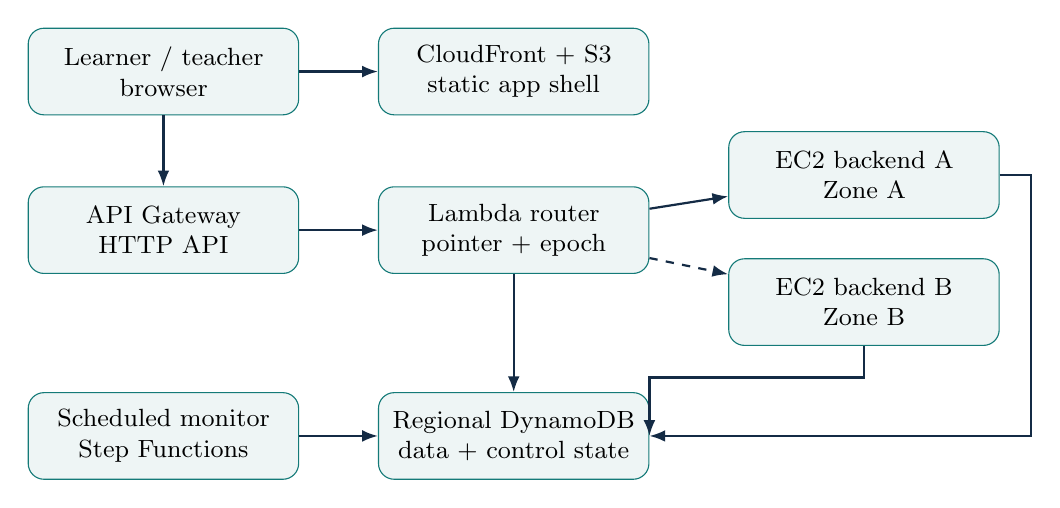
\begin{tikzpicture}[font=\small,box/.style={draw=teal,fill=pale,rounded corners=2mm,align=center,minimum height=11mm,text width=32mm},arrow/.style={-{Latex[length=2mm]},color=navy,thick}]
\node[box] (browser) {Learner / teacher\\browser};
\node[box,right=10mm of browser] (edge) {CloudFront + S3\\static app shell};
\node[box,below=9mm of browser] (gateway) {API Gateway\\HTTP API};
\node[box,right=10mm of gateway] (router) {Lambda router\\pointer + epoch};
\node[box,right=10mm of router,yshift=7mm] (a) {EC2 backend A\\Zone A};
\node[box,below=5mm of a] (b) {EC2 backend B\\Zone B};
\node[box,below=15mm of router] (ddb) {Regional DynamoDB\\data + control state};
\node[box,left=10mm of ddb] (monitor) {Scheduled monitor\\Step Functions};
\draw[arrow] (browser)--(edge);\draw[arrow] (browser)--(gateway);
\draw[arrow] (gateway)--(router);\draw[arrow] (router)--(a);
\draw[arrow,dashed] (router)--(b);\draw[arrow] (router)--(ddb);
\draw[arrow] (a.east)--++(4mm,0)|-(ddb.east);
\draw[arrow] (b.south)--++(0,-4mm)-|(ddb.east);
\draw[arrow] (monitor)--(ddb);
\end{tikzpicture}
\caption{Source-defined supported topology. The dashed route is the alternate selected backend after verified promotion. This diagram does not assert current cloud deployment or health.}
\end{figure}

The supported defaults target Sydney, \texttt{ap-southeast-2}. Regional resources must remain in the project's assigned selected Region. Archived cross-Region directories are not the supported deployment. No cloud resources were created, changed, inventoried or faulted during this audit.

\textbf{Evidence:} \src{go.mod}; \src{web/package.json}; \src{infra/demo/network.tf}; \src{infra/demo/lambda.tf}; \src{infra/demo/workflow.tf}; \src{docs/architecture.md}.
\clearpage

\section{Data model and integrity mechanisms}
\subsection{Single-table entities}
\begin{tabularx}{\textwidth}{@{}P{36mm}X@{}}\toprule Entity family & Purpose and relationships \\\midrule
User / email index & Profile, hash, role and session version; unique email lookup. \\
Exam / questions & Teacher/class assignment, availability, duration, attempt limits and weighted questions. \\
Draft / bank & Teacher-owned authoring material, reusable questions and publish state. \\
Attempt & Answers, start time, optimistic version and attempt number; earlier attempts archived on retake. \\
Submission / receipt & Canonical grade and final map; request-linked replay record and earlier attempt snapshots. \\
Outbox / audit & Reconciliation records and deduplicated audit summaries. \\
Classroom / member & Owner, shared code, roster, lookup records and email-bound invitations. \\
Board current / history & Latest scene pointer and versioned serialized snapshots. \\
Control / events & Active backend, monotonic epoch, paused/incident state and recovery evidence. \\\bottomrule\end{tabularx}
\subsection{Attempt and submission lifecycle}
\begin{enumerate}
\item The learner inspects read-only metadata. Begin/resume requests question delivery and records the server start when necessary.
\item The browser updates a user/exam/attempt-scoped local map and sends version-checked autosaves. Gaps remain around empty maps, overlapping requests and merge semantics (\issue{CQ-064}--\issue{CQ-069}).
\item Final submission creates or reloads a stored immutable request ID and answer snapshot. Retries retain the pair and transient failures preserve the pending intent.
\item The store commits a canonical submission with supporting receipt/outbox records. Routed writes include the active-backend/epoch condition in the transaction.
\item The browser confirms completion only after a matching receipt reference. Replay can recover that receipt even after the exam window closes.
\end{enumerate}
\subsection{Strengths and remaining boundaries}
Writer fencing is atomic with application mutation. Retakes carry explicit attempt identity, and tests cover replay and stale-attempt conditions. Membership writes use conditional transactions. These are implemented mechanisms, not future work.

Remaining work includes start/deadline integrity, mutable duration, draft revisions and cross-manager board ordering. DynamoDB limits a transaction to 100 unique items and an item to 400 KB, making question-count and scene-size contracts material concerns [1].

\textbf{Evidence:} \src{internal/model/model.go}; \src{internal/store/retakes.go}; \src{internal/store/store.go:182}; \src{internal/clusterstate/contract.go}; \src{internal/boards/persistence.go}.
\clearpage

\section{Recovery behavior and operational scope}
\subsection{Normal and degraded service}
The router loads the active pointer for each request and forwards writer metadata to that backend. It does not silently try the standby after a failed upstream request. Promotion depends on repeated capability observations and standby verification. Liveness and readiness are separate: a process can remain alive while its database capability is faulted.

An epoch change prevents the previously active writer from committing after promotion. Recovery includes public-route verification; rollback and failback retain monotonic control state. Submission retry identity stays stable across the disruption. Reconciliation can be repeated without intentionally duplicating downstream audit work.
\subsection{Local and cloud differences}
\begin{tabularx}{\textwidth}{@{}>{\raggedright\arraybackslash}p{30mm}>{\raggedright\arraybackslash}X>{\raggedright\arraybackslash}X@{}}\toprule Aspect & Local rehearsal & Supported cloud definition \\\midrule
Application failure & Separate HTTP listeners in one process & Two EC2 nodes in different Availability Zones \\
Data durability & Shared process memory & Regional DynamoDB \\
Monitoring & Local controller/probe loop & EventBridge plus Lambda/Step Functions \\
Frontend transport & Vite API/socket proxy & CloudFront shell, separate HTTPS HTTP API \\
Boards & Standalone API WebSocket collaboration & No promised board/WebSocket failover in the bounded HTTP demo \\\bottomrule\end{tabularx}

Complete selected-Region failure, a regional DynamoDB outage and an entire local process exit are outside the demonstrated boundary. The one-minute cloud schedule can add detection delay before the measured probe-to-public-verification duration; the cockpit already explains that distinction. Small throttling limits and retained paused resources also make this a faculty demonstration, not a classroom capacity claim.
\subsection{Operational improvements}
Preserve fencing and receipt behavior while adding observation freshness, scoped fault controls, backups and a verified restore procedure. Before private classroom board use, decide the sharing model and apply it consistently to sockets, history and export. Before expanding load, test simultaneous start, autosave and control traffic within approved project capacity and spend constraints.

\textbf{Evidence:} \src{internal/continuum/router.go}; \src{internal/continuum/supervisor.go}; \src{internal/continuum/verifier.go}; \src{statemachine/demo-failover.asl.json}; \src{infra/demo/workflow.tf:8}; \src{README.md}.
\clearpage

\section{Interface observations}
\begin{figure}[h!]\centering
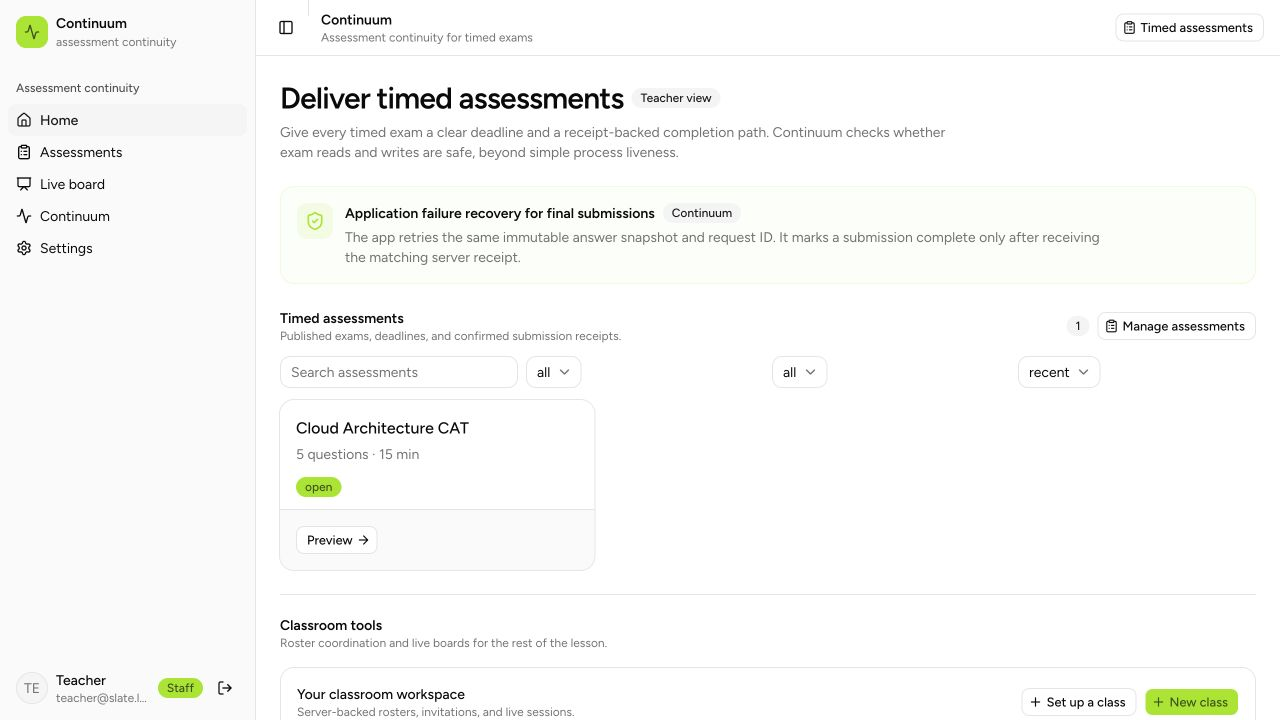
\includegraphics[width=\textwidth]{screenshots/teacher-home.png}
\caption{Teacher dashboard in an isolated local session. Closed filter triggers show internal values ``all'' and ``recent'' (\issue{CQ-107}). The identity is the synthetic local bootstrap teacher.}
\end{figure}
\begin{figure}[h!]\centering
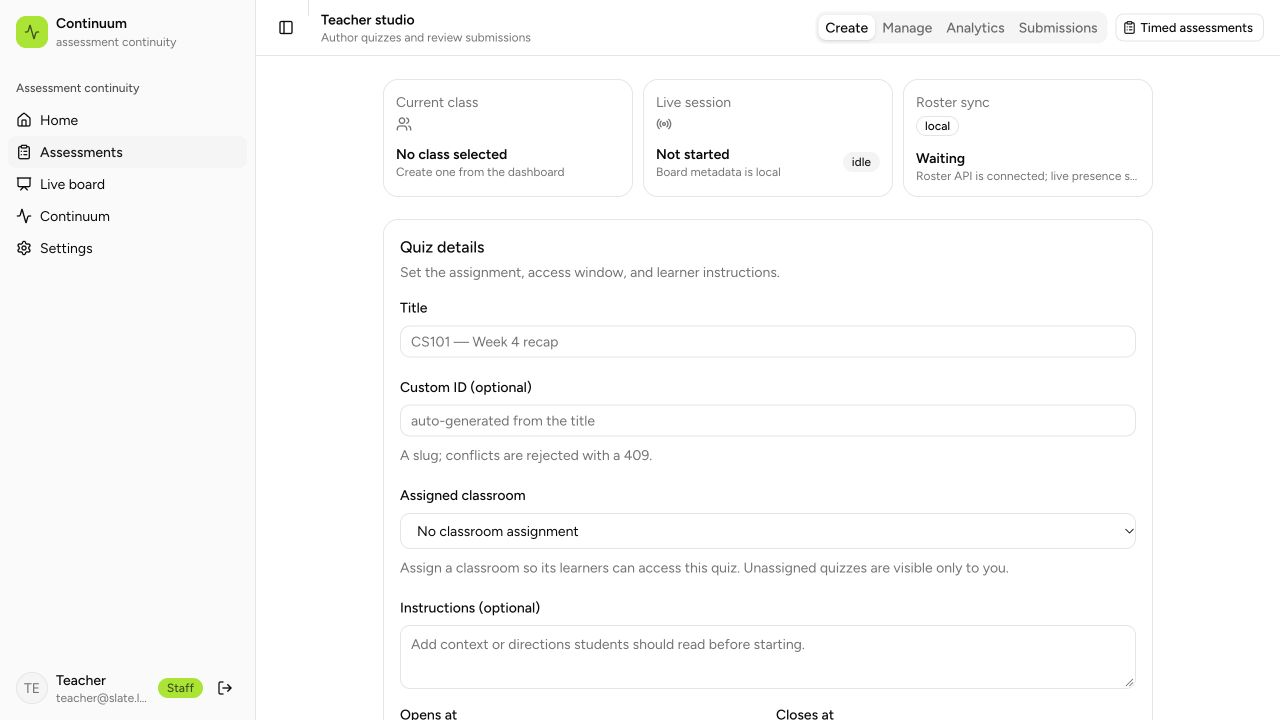
\includegraphics[width=\textwidth]{screenshots/teacher-studio.png}
\caption{Desktop teacher studio with an empty authoring form. Create/Manage/Analytics/Submissions are AppShell actions; source review shows those controls are hidden on narrow screens (\issue{CQ-106}). The screenshot itself is a desktop view.}
\end{figure}
\clearpage

\section{Verification results and audit method}
\subsection{Executed checks}
\begin{tabularx}{\textwidth}{@{}P{57mm}P{20mm}X@{}}\toprule Check & Outcome & Interpretation \\\midrule
\texttt{go test -race -timeout 30m ./...} & Failed & Two authentication clock tests failed. All other reported packages passed, including HTTP API, store, recovery and integration. \\
\texttt{go vet ./...} & Passed & No vet diagnostics. \\
\texttt{bun run typecheck} & Passed & TypeScript check completed. \\
\texttt{bun run lint} & Passed & ESLint completed. \\
\texttt{bun run test} & Passed & 27 test files, 167 tests. \\
\texttt{bun run build} & Passed & Client/server build and prerender completed, with large-chunk and route-export splitting warnings. \\
\texttt{bunx playwright test} & Passed & All 8 existing journeys; about 1.2 minutes. \\
Focused memory API probes & Completed & 17 observation cases; 16 register entries supported by probe evidence, with shared evidence for some entries. \\
Terraform / live AWS exercise & Not run & Configuration review only; no live cloud reproduction or capacity result is asserted. \\\bottomrule\end{tabularx}
\subsection{Method and evidence levels}
The review traced entrypoints through transport, domain rules, persistence and frontend state. It examined source, current guides, tests, supported Terraform and release scripts. Existing checks ran unchanged. Focused probes used \texttt{httptest} and an isolated memory store, with synthetic data and no AWS access. A browser session inspected the dashboard and teacher studio.

Every entry supplies a checked file/line, a trigger, consequence, fix and acceptance check. \texttt{findings.json} also preserves evidence labels, source lines and file SHA-256 values. Source-reviewed races and failure scenarios are reasoned findings, not executed concurrency/load tests. Hardening recommendations do not assert exploitation.
\subsection{Verification limits}
This is not a formal security assessment, full accessibility conformance review or benchmark. SMTP delivery, real DynamoDB behavior, live IAM permissions, backup restoration, multiple real devices and every browser/viewport were not exercised. No dependency vulnerability scan was run. Existing \texttt{docs/evidence} screenshots were treated as historical material, not new runtime proof.
\clearpage

\section{Selected reproduction evidence}
\begin{tabularx}{\textwidth}{@{}P{22mm}P{51mm}X@{}}\toprule Finding & Local probe & Actual outcome \\\midrule
\issue{CQ-018} & Submit to a one-minute exam before start & HTTP 200 committed receipt; score 1/1. \\
\issue{CQ-016} & Correct option under question key \texttt{00} & HTTP 200 receipt; score 0/1. \\
\issue{CQ-017} & Choice 99 for two-option question & HTTP 503: data layer unavailable. \\
\issue{CQ-020} & Change duration 15 to 1 after start & Same start; deadline moved earlier by 840,000 ms. \\
\issue{CQ-013} & Create with only \texttt{opens\_at=garbage} & HTTP 201; invalid boundary persisted. \\
\issue{CQ-021} & Close with late work enabled & Close succeeds; subsequent delivery returns 200. \\
\issue{CQ-030} & Reuse save ID with changed answers & HTTP 200 duplicate, earlier answer map returned. \\
\issue{CQ-036} & Frontend-equivalent board history path & HTTP 404 from isolated API. \\
\issue{CQ-038} & Restore by unrelated teacher & HTTP 200; no room-owner check. Hardening of the current shared-code model. \\
\issue{CQ-040} & Inspect restore response & Capitalized \texttt{Elements}/\texttt{Peers}; client expects \texttt{elements}. \\
\issue{CQ-008} & Zero-hit rate limit & Recovered index-out-of-range panic. \\\bottomrule\end{tabularx}
\subsection{Existing Go test failures}
\path{TestPasswordChangeAndResetRevokeSessionsAndEnforceSingleUseExpiry} failed at \src{internal/auth/qol_test.go:48} with ``invalid or expired session.'' Token issuance used 11 October while parsing used current time. \path{TestPasswordUpdatesInvalidateEveryOutstandingResetToken} failed at line 135 with ``invalid password reset record'' because the store clock was not advanced with the service clock. Both belong to \issue{CQ-119}; neither by itself proves a production reset regression.
\subsection{Reproduction command}
From the repository root:
\begin{quote}\small\ttfamily go run ./docs/reports/continuum-audit-2026-10-23/probes\end{quote}
The helper prints synthetic observation JSON and creates no external resources. Saved output is \src{evidence/focused-probes.json} relative to the report project.
\clearpage

\section{Prioritized implementation plan}
\subsection{First batch: core correctness}
\begin{tabularx}{\textwidth}{@{}P{25mm}Xp{38mm}@{}}\toprule Batch & Concrete outcome & References \\\midrule
Attempt integrity & Require a start, preserve deadlines, canonicalize answer keys and define hard close. & \issue{CQ-016}, \issue{CQ-018}, \issue{CQ-020}, \issue{CQ-021} \\
Learner saves & Serialize saves, persist empty maps, track saved generations and retain clear/merge intent. & \issue{CQ-064}--\issue{CQ-069} \\
Board contracts & Align resource prefixes and response DTOs before relying on history/export. & \issue{CQ-036}, \issue{CQ-040} \\
Authoring integrity & Version saves/publish and condition exam creation/updates. & \issue{CQ-026}--\issue{CQ-028}, \issue{CQ-033} \\
Usable surfaces & Restore essential mobile actions and deterministic clock tests. & \issue{CQ-106}, \issue{CQ-119} \\\bottomrule\end{tabularx}
\subsection{Second batch: identity and collaboration}
Resolve whether class boards are private, code-accessible or deliberately public to signed-in users. Encode that decision using stable identity and ownership across read, restore and drawing controls. Address operator-token persistence, email verification, refresh resilience and trusted-client rate limiting. Preserve epoch fencing while adding monotonic board persistence and bounded peer queues.
\subsection{Third batch: recovery and authoring quality}
Add acknowledged board revisions and recoverable outgoing mutations. Make storage failures honest, link local drafts to server identity and expose bank/invitation retries. Retrieve earlier receipts, define timeout finalization and improve keyboard, countdown and printing behavior.
\subsection{Fourth batch: delivery and operational readiness}
Add browser checks to CI, retain old frontend assets, separate web releases from runtime changes and implement a tested backup/restore policy. Expand capacity after representative load tests; current limits can remain suitable for a small rehearsal when that boundary is explicit.

\textbf{Completion rule.} Close an issue when its acceptance check passes on relevant persistence paths, with browser verification for visible behavior. Existing tests alone do not establish that a newly uncovered edge case is fixed. Effort estimates depend on product policy, production scope and migration choices and are not invented here.
\clearpage

\section{Finding classification and navigation}
\begin{tabularx}{\textwidth}{Xr}\toprule Category & Items \\\midrule
Identity, security and HTTP boundaries & 12 \\
Assessment API, grading and persistence & 23 \\
Shared board correctness and collaboration & 28 \\
Learner workflow, recovery and accessibility & 16 \\
Teacher authoring and local data recovery & 16 \\
Classroom coordination and invitation behavior & 10 \\
Interface polish, operations, delivery and verification & 15 \\\bottomrule\end{tabularx}

\subsection{Priority definitions}
\begin{tabularx}{\textwidth}{@{}P{16mm}P{16mm}X@{}}\toprule Priority & Count & Meaning \\\midrule
P1 & 45 & Early repair: integrity, lost work, core blockage, significant authorization boundary or failed verification gate. \\
P2 & 67 & Planned repair: reliability, recovery clarity, hardening, performance, accessibility or workflow inconsistency. \\
P3 & 8 & Presentation, documentation or lower-impact refinement. \\\bottomrule\end{tabularx}
\subsection{Kinds and interpretation}
\textbf{Defect} identifies an implementation inconsistency with a concrete undesired result. \textbf{Hardening} strengthens a defensive boundary for broader use. \textbf{Policy gap} needs a product decision. \textbf{Missing capability} names an absent recovery/workflow path. Other kinds are labeled directly.

The register has 68 defects, 28 hardening items, 4 policy gaps, 7 missing capabilities, 2 accessibility items, 7 polish items, and one each for performance, demo capacity, CI verification and documentation. These are not 120 independently reproduced runtime bugs.
\subsection{Evidence package}
\begin{itemize}
\item \texttt{BACKLOG.md} and \texttt{findings.csv}: readable/sortable planning register.
\item \texttt{findings.json}: structured entries, evidence labels and source hashes.
\item \texttt{probes/main.go}: repeatable isolated observations.
\item \texttt{evidence/}: Go, vet, browser and focused-probe results plus verification summary.
\item \texttt{main.tex}, \texttt{findings.tex}, \texttt{summary-tables.tex}: editable report source.
\end{itemize}
\section{Detailed issue register}
The following pages contain all 120 entries. Source locators refer to the reviewed baseline; later implementation changes may move those lines. Stable issue IDs match the CSV and JSON.
\clearpage
\section*{Issue register: CQ-001 to CQ-004}
\phantomsection\addcontentsline{toc}{subsection}{Identity, security and HTTP boundaries}
\begin{finding}{CQ-001}{P1}{Known development secrets are accepted at startup}
\textbf{Hardening} $\cdot$ Source review\par
\textbf{Source}\quad\path{internal/config/config.go:66}\par
Starting the API without explicit secrets uses a published admin token and JWT signing key. An accidentally exposed development instance therefore has predictable credentials.\par
\textbf{Fix.} Require explicit strong secrets outside an explicit local development mode.\par
\textbf{Accept when.} Production-mode startup rejects missing, default and empty secrets; isolated local mode remains convenient.
\end{finding}
\begin{finding}{CQ-002}{P1}{Signing out leaves the administrator token behind}
\textbf{Defect} $\cdot$ Source review\par
\textbf{Source}\quad\path{web/src/lib/auth.ts:107}\par
clearAuth removes login state but leaves slate.admin-token in localStorage. On a shared browser the next person can retain cockpit authority after a visible sign-out.\par
\textbf{Fix.} Clear or separately lock the admin session on sign-out; use a short-lived scoped operator session.\par
\textbf{Accept when.} Sign out with an admin token present; reopening /ops requires operator authentication.
\end{finding}
\begin{finding}{CQ-003}{P1}{A temporary refresh outage destroys the login session}
\textbf{Defect} $\cdot$ Source review\par
\textbf{Source}\quad\path{web/src/lib/api.ts:91}\par
Every non-success refresh response clears authentication, including 503 and 429. A backend recovery or throttling event signs learners out even though their refresh token may remain valid.\par
\textbf{Fix.} Clear the session only for definitive token rejection; retain it on transient failures.\par
\textbf{Accept when.} Force refresh to return 503 and 429; stored authentication remains and a later request recovers.
\end{finding}
\begin{finding}{CQ-004}{P2}{Refresh tokens remain reusable until expiry}
\textbf{Hardening} $\cdot$ Source review\par
\textbf{Source}\quad\path{internal/httpapi/server.go:391}\par
Refresh issues replacement tokens without consuming the old refresh token. A copied token can be replayed repeatedly during its lifetime unless a password change increments the session version.\par
\textbf{Fix.} Add rotating refresh sessions with reuse detection and revocation.\par
\textbf{Accept when.} Refresh once, replay the old token, and verify the old token is rejected without invalidating unrelated sessions.
\end{finding}
\clearpage
\section*{Issue register: CQ-005 to CQ-008}
\begin{finding}{CQ-005}{P1}{Email-bound invitations trust unverified addresses}
\textbf{Hardening} $\cdot$ Source review\par
\textbf{Source}\quad\path{internal/httpapi/server.go:309}\par
Registration immediately trusts the submitted email and returns a session. Possession of an invitation code plus a newly claimed matching email is enough to join; mailbox ownership is never established.\par
\textbf{Fix.} Verify mailbox ownership before accepting email-bound invitations.\par
\textbf{Accept when.} A newly registered unverified address cannot consume an invitation until verification completes.
\end{finding}
\begin{finding}{CQ-006}{P1}{Credential recovery and password changes have no route limits}
\textbf{Hardening} $\cdot$ Source review\par
\textbf{Source}\quad\path{internal/middleware/middleware.go:219}\par
The limiter registers only login and registration. Forgot-password, reset-password and change-password can repeatedly trigger email delivery, token records or expensive bcrypt work.\par
\textbf{Fix.} Apply bounded per-origin and per-identity limits to recovery and password endpoints.\par
\textbf{Accept when.} Repeated recovery and password requests receive 429 while normal sign-in and exam traffic continue.
\end{finding}
\begin{finding}{CQ-007}{P1}{Proxy traffic shares the same login-rate bucket}
\textbf{Defect} $\cdot$ Source review\par
\textbf{Source}\quad\path{internal/middleware/middleware.go:226}\par
Rate limiting keys off the immediate remote host. The public router forwards requests from itself, so many learners reaching one backend can share a small login bucket. The Gateway adapter also omits source identity.\par
\textbf{Fix.} Propagate a verified client identity through the trusted router and enforce limits at the appropriate boundary.\par
\textbf{Accept when.} Several independent clients can each use their allowance through the router; spoofed forwarded headers do not bypass limits.
\end{finding}
\begin{finding}{CQ-008}{P1}{Setting a rate limit to zero panics}
\textbf{Defect} $\cdot$ Reproduced (isolated memory API)\par
\textbf{Source}\quad\path{internal/middleware/middleware.go:178}\par
MaxHits equal to zero enters the rejection branch with an empty hit slice and reads hits[0]. The focused probe reproduced an index-out-of-range panic.\par
\textbf{Fix.} Define zero semantics explicitly and validate configuration before constructing the limiter.\par
\textbf{Accept when.} Zero configured hits produce a controlled rejection or startup error without a panic.
\end{finding}
\clearpage
\section*{Issue register: CQ-009 to CQ-012}
\begin{finding}{CQ-009}{P2}{Negative security settings silently disable protection}
\textbf{Defect} $\cdot$ Reproduced (isolated memory API)\par
\textbf{Source}\quad\path{internal/config/config.go:153}\par
Numeric parsing accepts negative login and registration limits; Allow interprets a negative maximum as unlimited. Other durations and thresholds also lack range validation.\par
\textbf{Fix.} Validate semantic ranges and offer a named, explicit development override for unlimited limits.\par
\textbf{Accept when.} Negative limits, nonpositive token lifetimes and invalid threshold values fail configuration loading.
\end{finding}
\begin{finding}{CQ-010}{P2}{Registration counts name bytes while profile editing counts characters}
\textbf{Defect} $\cdot$ Reproduced (isolated memory API)\par
\textbf{Source}\quad\path{internal/httpapi/server.go:2146}\par
Registration rejects names over 60 UTF-8 bytes, while UpdateName allows 60 Unicode code points. The probe rejected a name containing only 21 CJK characters.\par
\textbf{Fix.} Use one character-count policy across creation, profile changes and UI hints.\par
\textbf{Accept when.} The same 60-character Unicode name can be registered and subsequently edited.
\end{finding}
\begin{finding}{CQ-011}{P1}{The standalone API has no request-body budget}
\textbf{Hardening} $\cdot$ Source review\par
\textbf{Source}\quad\path{internal/httpapi/server.go:2110}\par
JSON decoding reads an unbounded body and the direct server sets only header and idle timeouts. The Continuum router has a size limit, but standalone API deployments bypass it.\par
\textbf{Fix.} Limit request bodies and body-read time at the API boundary, with separate intentional board limits.\par
\textbf{Accept when.} Oversized JSON returns 413 and a stalled body times out without retaining an unbounded handler.
\end{finding}
\begin{finding}{CQ-012}{P2}{Sensitive API responses omit explicit no-store policy}
\textbf{Hardening} $\cdot$ Reproduced (isolated memory API)\par
\textbf{Source}\quad\path{internal/httpapi/server.go:2126}\par
Identity, results, roster and token responses use the generic writer without Cache-Control. The focused identity probe observed an empty cache policy. Browser or intermediary defaults are left to decide retention.\par
\textbf{Fix.} Emit an explicit no-store policy for identity, credentials and private assessment data.\par
\textbf{Accept when.} Sensitive responses consistently carry the intended no-store header through local and cloud routing.
\end{finding}
\clearpage
\section*{Issue register: CQ-013 to CQ-016}
\phantomsection\addcontentsline{toc}{subsection}{Assessment API, grading and persistence}
\begin{finding}{CQ-013}{P1}{A single malformed availability boundary is accepted}
\textbf{Defect} $\cdot$ Reproduced (isolated memory API)\par
\textbf{Source}\quad\path{internal/httpapi/server.go:2194}\par
createExam validates timestamps only when both are supplied. The probe created an exam with opens\_at set to garbage; EnforceWindow later ignores invalid stored boundaries.\par
\textbf{Fix.} Validate each nonempty timestamp independently before comparing the pair.\par
\textbf{Accept when.} Malformed opening-only and closing-only payloads fail with a field-level 4xx response.
\end{finding}
\begin{finding}{CQ-014}{P2}{Creation and editing enforce different text limits}
\textbf{Defect} $\cdot$ Source review\par
\textbf{Source}\quad\path{internal/httpapi/server.go:2153}\par
Direct exam creation does not apply the title, instruction and feedback limits used by other authoring routes or updates. A newly created value can be impossible to save unchanged later.\par
\textbf{Fix.} Centralize the assessment validation contract for all creation and update paths.\par
\textbf{Accept when.} Identical title, instruction and feedback boundaries are accepted or rejected consistently across endpoints.
\end{finding}
\begin{finding}{CQ-015}{P1}{Direct exam creation can exceed the transaction budget}
\textbf{Defect} $\cdot$ Source review\par
\textbf{Source}\quad\path{internal/store/store.go:402}\par
EnsureExam emits one metadata write plus one per question, and routed writes add a fencing condition. The direct create route does not bound question count, so an accepted payload can exceed DynamoDB's transaction limit.\par
\textbf{Fix.} Enforce the effective atomic question budget before persistence and return a useful validation message.\par
\textbf{Accept when.} At and above the supported question boundary, memory and DynamoDB paths return equivalent outcomes.
\end{finding}
\begin{finding}{CQ-016}{P1}{Noncanonical question keys validate but grade incorrectly}
\textbf{Defect} $\cdot$ Reproduced (isolated memory API)\par
\textbf{Source}\quad\path{internal/exams/exams.go:450}\par
validateAnswers uses Atoi, accepting keys such as 00 or +0, while grading looks up canonical decimal keys. The probe submitted the correct choice under 00 and received zero points.\par
\textbf{Fix.} Reject noncanonical keys or canonicalize with collision detection before validation and grading.\par
\textbf{Accept when.} Alternate numeric spellings never silently become an accepted but ungraded answer.
\end{finding}
\clearpage
\section*{Issue register: CQ-017 to CQ-020}
\begin{finding}{CQ-017}{P2}{Invalid answer payloads look like service outages}
\textbf{Defect} $\cdot$ Reproduced (isolated memory API)\par
\textbf{Source}\quad\path{internal/httpapi/server.go:2070}\par
validateAnswers returns ordinary formatted errors, while writeExamError maps unknown errors to 503. The probe sent an out-of-range choice and received data layer unavailable.\par
\textbf{Fix.} Return a typed validation error and map it to 400 or 422.\par
\textbf{Accept when.} Invalid question keys, invalid choices and negative save versions produce clear nonretryable client errors.
\end{finding}
\begin{finding}{CQ-018}{P1}{A timed assessment accepts submission without a started attempt}
\textbf{Defect} $\cdot$ Reproduced (isolated memory API)\par
\textbf{Source}\quad\path{internal/exams/exams.go:226}\par
The deadline check rejects only a non-nil existing deadline. A learner can call the final submit endpoint before the start route; the focused timed-exam probe committed successfully.\par
\textbf{Fix.} Require an existing started attempt for timed submissions and bind its identity at commit.\par
\textbf{Accept when.} Submission without a start is rejected; a legitimately started attempt retains the same deadline.
\end{finding}
\begin{finding}{CQ-019}{P1}{Teachers can enter the learner submission pipeline}
\textbf{Defect} $\cdot$ Reproduced (isolated memory API)\par
\textbf{Source}\quad\path{internal/exams/exams.go:175}\par
Submission requires a user but does not require the student role. A teacher's direct submit request committed a scored submission in the probe, potentially contaminating learner analytics.\par
\textbf{Fix.} Restrict learner save/start/submit routes to students or provide a separate explicitly excluded preview mode.\par
\textbf{Accept when.} Teacher preview does not create attempts or grade rows counted as learner submissions.
\end{finding}
\begin{finding}{CQ-020}{P1}{Editing duration changes deadlines for attempts already running}
\textbf{Defect} $\cdot$ Reproduced (isolated memory API)\par
\textbf{Source}\quad\path{internal/store/store.go:2938}\par
Deadlines are recomputed from current exam duration rather than stored with the attempt. The probe shortened duration from 15 to 1 minute and observed the active deadline move by 14 minutes.\par
\textbf{Fix.} Persist each attempt's authoritative deadline and define explicit rules for permitted extensions.\par
\textbf{Accept when.} Shortening an exam's default duration does not retroactively shorten existing attempts.
\end{finding}
\clearpage
\section*{Issue register: CQ-021 to CQ-024}
\begin{finding}{CQ-021}{P1}{Close does not stop an assessment that allows late work}
\textbf{Defect} $\cdot$ Reproduced (isolated memory API)\par
\textbf{Source}\quad\path{internal/httpapi/server.go:1625}\par
closeExam sets closes\_at to now but leaves allow\_late enabled. EnforceWindow still admits late work; the focused probe could reopen the learner delivery route after Close succeeded.\par
\textbf{Fix.} Make the close action explicitly stop acceptance, or rename it and provide a separate hard-close action.\par
\textbf{Accept when.} After a hard close, new starts and final submissions are rejected even when late work was previously enabled.
\end{finding}
\begin{finding}{CQ-022}{P1}{Immediate answer review can reveal answers before retakes}
\textbf{Policy gap} $\cdot$ Source review\par
\textbf{Source}\quad\path{internal/httpapi/server.go:955}\par
Every result exposes correct answers and feedback immediately. An exam with multiple or unlimited attempts lets a learner review the answer key and then start another scored attempt.\par
\textbf{Fix.} Add a teacher-controlled review-release policy and explain how it interacts with retakes.\par
\textbf{Accept when.} With review delayed, learners can see their receipt and permitted score without receiving the answer key.
\end{finding}
\begin{finding}{CQ-023}{P2}{Losing classroom access also removes receipt access}
\textbf{Policy gap} $\cdot$ Source review\par
\textbf{Source}\quad\path{internal/httpapi/server.go:934}\par
Result access rechecks current enrollment and current classroom assignment. A removed learner or a learner whose exam is reassigned loses access to an already committed result.\par
\textbf{Fix.} Authorize historical receipts by submission ownership while enforcing current membership for new work.\par
\textbf{Accept when.} Remove a submitted learner from a class; their own existing receipt remains readable.
\end{finding}
\begin{finding}{CQ-024}{P2}{Earlier attempt receipts have no learner retrieval route}
\textbf{Missing capability} $\cdot$ Source review\par
\textbf{Source}\quad\path{internal/httpapi/server.go:937}\par
Retakes archive previous submission snapshots, but /result reads only the latest submission and accepts no attempt selector. The UI promise that earlier receipts remain recorded has no history browsing path.\par
\textbf{Fix.} Expose a user-scoped attempt history and receipt route, then link it from results.\par
\textbf{Accept when.} After two completed attempts, both receipts and their answer reviews can be retrieved independently.
\end{finding}
\clearpage
\section*{Issue register: CQ-025 to CQ-028}
\begin{finding}{CQ-025}{P2}{Result review silently disappears on a question-read error}
\textbf{Defect} $\cdot$ Source review\par
\textbf{Source}\quad\path{internal/httpapi/server.go:946}\par
The result handler discards GetExam errors and returns 200 with an empty review. A data-layer failure becomes indistinguishable from a successful receipt lacking question detail.\par
\textbf{Fix.} Preserve the confirmed receipt but explicitly expose review availability and a retry path.\par
\textbf{Accept when.} Inject a question read failure; the client sees a confirmed receipt plus a clear incomplete-review state.
\end{finding}
\begin{finding}{CQ-026}{P1}{Concurrent direct creates can overwrite an assessment}
\textbf{Defect} $\cdot$ Source review\par
\textbf{Source}\quad\path{internal/httpapi/server.go:1431}\par
The create route checks absence before EnsureExam, whose metadata and question puts are unconditional. Two requests can pass the check together; one can replace the other's owner and content.\par
\textbf{Fix.} Use a conditional create transaction, mapping the loser to 409.\par
\textbf{Accept when.} Concurrent creates of the same normalized ID produce exactly one winner and no mixed question set.
\end{finding}
\begin{finding}{CQ-027}{P1}{Draft updates have no cross-tab version check}
\textbf{Defect} $\cdot$ Source review\par
\textbf{Source}\quad\path{internal/store/store.go:795}\par
UpdateQuizDraft conditions on owner and status but not a draft revision. Serialized autosave within one component cannot prevent another tab or device from overwriting newer edits.\par
\textbf{Fix.} Add a draft revision and require the version being edited on every update.\par
\textbf{Accept when.} Two editors save from the same revision; the second receives a recoverable conflict instead of overwriting content.
\end{finding}
\begin{finding}{CQ-028}{P1}{Publishing can use a stale draft snapshot}
\textbf{Defect} $\cdot$ Source review\par
\textbf{Source}\quad\path{internal/store/store.go:843}\par
Publish reads the draft and later conditions only on owner/status. A concurrent autosave can update questions while status remains draft, allowing an older read to be published and marked current.\par
\textbf{Fix.} Tie publish to a draft revision or content digest in the same transaction.\par
\textbf{Accept when.} Hold publication after its read, save a newer draft, then resume; publication rejects the stale version.
\end{finding}
\clearpage
\section*{Issue register: CQ-029 to CQ-032}
\begin{finding}{CQ-029}{P2}{A 98-question cloud draft cannot be published}
\textbf{Defect} $\cdot$ Source review\par
\textbf{Source}\quad\path{internal/store/store.go:788}\par
Updates allow up to 98 questions, but PublishQuizDraft rejects more than 97. Memory-backed publishing follows a different path, so local success can conceal this cloud-only boundary.\par
\textbf{Fix.} Align authoring, storage and publishing limits and display the supported maximum.\par
\textbf{Accept when.} Save and publish the largest allowed draft on both backends; the next question receives the same validation error.
\end{finding}
\begin{finding}{CQ-030}{P2}{Autosave deduplication does not bind the answer snapshot}
\textbf{Defect} $\cdot$ Reproduced (isolated memory API)\par
\textbf{Source}\quad\path{internal/exams/exams.go:361}\par
Reusing the last save request ID returns duplicate before comparing payloads. The probe reused an ID with changed answers and received a successful duplicate response containing the older answers.\par
\textbf{Fix.} Store a payload digest and reject request-ID reuse with different answers.\par
\textbf{Accept when.} Same-ID same-payload retry is idempotent; same-ID changed-payload retry returns a conflict.
\end{finding}
\begin{finding}{CQ-031}{P1}{Deadline validation is separated from the final write}
\textbf{Hardening} $\cdot$ Source review\par
\textbf{Source}\quad\path{internal/exams/exams.go:231}\par
The service checks time before calling the store; the submission transaction fences the writer but does not check an immutable deadline or schedule revision. A delayed request can cross a closing boundary after validation.\par
\textbf{Fix.} Define commit-time deadline semantics and enforce a stored deadline or validated revision in the atomic write path.\par
\textbf{Accept when.} A deliberately delayed final write crossing the allowed boundary has a deterministic documented outcome.
\end{finding}
\begin{finding}{CQ-032}{P2}{Assessment deletion leaves related data without a lifecycle policy}
\textbf{Hardening} $\cdot$ Source review\par
\textbf{Source}\quad\path{internal/store/store.go:1423}\par
DeleteExam removes only EXAM\# rows. Attempts, submissions, request receipts, audit/outbox data and published draft records use other partitions and remain after the UI reports deletion.\par
\textbf{Fix.} Define archival and erasure semantics, then implement indexed cleanup or explicitly label archive behavior.\par
\textbf{Accept when.} Delete or archive a populated assessment and verify each related data family follows the documented retention policy.
\end{finding}
\clearpage
\section*{Issue register: CQ-033 to CQ-036}
\begin{finding}{CQ-033}{P1}{A concurrent metadata patch can resurrect a deleted exam}
\textbf{Defect} $\cdot$ Source review\par
\textbf{Source}\quad\path{internal/store/store.go:977}\par
UpdateExamWindow uses an update without an existence condition. After staff authorization reads metadata, a concurrent delete can remove it and a later update can recreate a partial META row without questions.\par
\textbf{Fix.} Require metadata existence and a revision in the update condition.\par
\textbf{Accept when.} Race deletion with a metadata patch; no partial assessment reappears.
\end{finding}
\begin{finding}{CQ-034}{P2}{The catalog scans globally and performs serial per-exam reads}
\textbf{Performance} $\cdot$ Source review\par
\textbf{Source}\quad\path{internal/httpapi/server.go:970}\par
listExams requests every exam, checks visibility one by one and loads attempt/submission state per learner. Response cost grows with the entire catalog, including exams the caller cannot see.\par
\textbf{Fix.} Query owner/member-visible indexes, paginate, and batch attempt enrichment.\par
\textbf{Accept when.} Measure catalog queries with many unrelated classes; work scales with the requested visible page.
\end{finding}
\begin{finding}{CQ-035}{P2}{Analytics silently stop after 1,000 learners}
\textbf{Defect} $\cdot$ Source review\par
\textbf{Source}\quad\path{internal/httpapi/server.go:1657}\par
examResults requests at most 1,000 latest submission rows and reports count and averages as if the list were complete. No continuation cursor or truncation signal reaches the teacher.\par
\textbf{Fix.} Paginate results and compute aggregates over the intended full population.\par
\textbf{Accept when.} More than 1,000 submissions produce complete aggregates or a clearly labeled partial page.
\end{finding}
\phantomsection\addcontentsline{toc}{subsection}{Shared board correctness and collaboration}
\begin{finding}{CQ-036}{P1}{Board history and export URLs do not match the API}
\textbf{Defect} $\cdot$ Reproduced (isolated memory API)\par
\textbf{Source}\quad\path{web/src/lib/api.ts:216}\par
The client calls /boards under BASE. The Vite proxy removes /api, while the server mounts history/export/restore only at /api/boards. Cloud BASE also leads to /boards. The focused client-path probe returned 404.\par
\textbf{Fix.} Choose one canonical board resource prefix and support it consistently in the client, proxy and API.\par
\textbf{Accept when.} History, export and restore succeed through both the documented local frontend and deployed API base.
\end{finding}
\clearpage
\section*{Issue register: CQ-037 to CQ-040}
\begin{finding}{CQ-037}{P1}{Any signed-in learner can read a known room's history}
\textbf{Hardening} $\cdot$ Reproduced (isolated memory API)\par
\textbf{Source}\quad\path{internal/httpapi/server.go:1007}\par
History and export require only a current user, without room ownership, membership or an explicit room capability. The focused unrelated-learner probe read another room's content and version list.\par
\textbf{Fix.} Define the room sharing boundary and enforce membership or a deliberate share capability on read operations.\par
\textbf{Accept when.} An unrelated signed-in learner cannot enumerate versions or export content from a private class board.
\end{finding}
\begin{finding}{CQ-038}{P1}{Any teacher can restore any known board}
\textbf{Hardening} $\cdot$ Reproduced (isolated memory API)\par
\textbf{Source}\quad\path{internal/httpapi/server.go:1042}\par
Restore requires the global staff role, without checking which teacher owns the room. The focused unrelated-teacher probe restored a room successfully. Room IDs therefore act as broad administrative capabilities.\par
\textbf{Fix.} Associate rooms with owners/classes and authorize destructive history operations against that relationship.\par
\textbf{Accept when.} A teacher from another class gets 403 on restore; the owning teacher can restore normally.
\end{finding}
\begin{finding}{CQ-039}{P1}{Drawing permissions are controlled by any teacher in a room}
\textbf{Hardening} $\cdot$ Source review\par
\textbf{Source}\quad\path{internal/boards/protocol.go:154}\par
The WebSocket permission branch checks only the teacher role, and Identity carries no stable user or class identity. Any teacher who knows a room code can enable or disable its learner drawing.\par
\textbf{Fix.} Include stable authenticated identity and verify the room's controlling teacher for permission changes.\par
\textbf{Accept when.} An unrelated teacher can participate only with their granted room role and cannot change room permissions.
\end{finding}
\begin{finding}{CQ-040}{P1}{Restore returns capitalized element fields that the client does not read}
\textbf{Defect} $\cdot$ Reproduced (isolated memory API)\par
\textbf{Source}\quad\path{internal/boards/manager.go:61}\par
RoomSnapshot exports Peers and Elements without JSON tags. The REST restore probe returned Elements, but api.boardRestore and BoardHistoryDialog expect elements. The callback therefore receives undefined.\par
\textbf{Fix.} Return a tagged response DTO matching the client contract and validate it at the boundary.\par
\textbf{Accept when.} Restore returns a lowercase elements array, and the restoring client's canvas updates even without a socket event.
\end{finding}
\clearpage
\section*{Issue register: CQ-041 to CQ-044}
\begin{finding}{CQ-041}{P1}{Connected board sessions survive token expiry and password revocation}
\textbf{Hardening} $\cdot$ Source review\par
\textbf{Source}\quad\path{internal/boards/http.go:105}\par
Authentication is performed once at the WebSocket handshake. Subsequent frames use the original identity indefinitely, so token expiry or a password change does not revoke an already connected board socket.\par
\textbf{Fix.} Bound socket authorization lifetime and revalidate or close sessions after revocation.\par
\textbf{Accept when.} Revoke a learner's session while connected; further board mutations are refused within the defined interval.
\end{finding}
\begin{finding}{CQ-042}{P2}{Board bearer tokens travel in the URL}
\textbf{Hardening} $\cdot$ Source review\par
\textbf{Source}\quad\path{web/src/lib/api.ts:385}\par
The access token is appended to the WebSocket query string. URLs can be retained by infrastructure request logs and debugging tools, increasing the credential exposure surface.\par
\textbf{Fix.} Exchange the session for a short-lived room ticket and redact sensitive query fields in logs.\par
\textbf{Accept when.} Connection URLs contain only short-lived scoped tickets, and logs do not retain reusable access tokens.
\end{finding}
\begin{finding}{CQ-043}{P1}{One slow socket can block unrelated board rooms}
\textbf{Hardening} $\cdot$ Source review\par
\textbf{Source}\quad\path{internal/boards/manager.go:454}\par
Broadcast writes to peers serially. The socket has no write deadline, and element handling holds the manager-wide control lock while broadcasting. A blocked recipient can stall later traffic across rooms.\par
\textbf{Fix.} Use bounded per-peer send queues, write deadlines and room-level serialization.\par
\textbf{Accept when.} Stall one peer's reads; healthy peers in that and another room continue receiving updates.
\end{finding}
\begin{finding}{CQ-044}{P2}{Element and room growth are not bounded}
\textbf{Hardening} $\cdot$ Source review\par
\textbf{Source}\quad\path{internal/boards/manager.go:279}\par
Per-frame byte limits do not bound the total number of accepted element IDs, room size or room creation. A signed-in client can accumulate many valid batches and exhaust process memory.\par
\textbf{Fix.} Add room, element, byte and per-identity quotas with clear rejection signals.\par
\textbf{Accept when.} Many small valid frames eventually hit a controlled room limit without exhausting memory or affecting other rooms.
\end{finding}
\clearpage
\section*{Issue register: CQ-045 to CQ-048}
\begin{finding}{CQ-045}{P1}{Full board snapshots can outgrow a DynamoDB item}
\textbf{Hardening} $\cdot$ Source review\par
\textbf{Source}\quad\path{internal/store/board_store.go:102}\par
Each complete board is serialized into snapshot\_json in both current and history records. There is no preflight size limit or blob-storage path when a scene approaches DynamoDB's 400 KB item maximum.\par
\textbf{Fix.} Keep large payloads in object storage or chunk them, and surface limits before accepting unsavable scenes.\par
\textbf{Accept when.} Save a scene near and above the item-size boundary; durability remains explicit and predictable.
\end{finding}
\begin{finding}{CQ-046}{P1}{Board persistence can overwrite newer history with an older revision}
\textbf{Hardening} $\cdot$ Source review\par
\textbf{Source}\quad\path{internal/store/board_store.go:117}\par
Current and history are unconditional puts. Serialization exists only inside one Manager; separate processes or out-of-order explicit saves can replace a newer current pointer or overwrite the same history key.\par
\textbf{Fix.} Add monotonic current-version conditions and immutable history conditions.\par
\textbf{Accept when.} Competing saves of older/newer or equal versions cannot roll back current state or rewrite an existing history record.
\end{finding}
\begin{finding}{CQ-047}{P2}{Peers receive raw element values that the server did not accept}
\textbf{Defect} $\cdot$ Source review\par
\textbf{Source}\quad\path{internal/boards/protocol.go:138}\par
The server filters maps and absorbs accepted versions, then broadcasts the original values list if any element changed. Mixed batches can forward invalid or rejected elements that are absent from authoritative server state.\par
\textbf{Fix.} Broadcast the normalized accepted element set or the authoritative merged result.\par
\textbf{Accept when.} Mixed valid/invalid/stale batches leave sender, peers and a reloaded snapshot consistent.
\end{finding}
\begin{finding}{CQ-048}{P2}{A transient snapshot failure has no automatic recovery attempt}
\textbf{Hardening} $\cdot$ Source review\par
\textbf{Source}\quad\path{internal/boards/persistence.go:562}\par
Failed snapshots are retained without a timer. This avoids retrying stale fenced epochs, but a transient failure on a valid writer can remain unsaved indefinitely unless another edit or explicit flush occurs.\par
\textbf{Fix.} Retry eligible transient errors with bounded backoff while stopping retries for fenced writers.\par
\textbf{Accept when.} Fail one persistence call, stop drawing, restore storage, and verify the latest valid snapshot becomes durable.
\end{finding}
\clearpage
\section*{Issue register: CQ-049 to CQ-052}
\begin{finding}{CQ-049}{P2}{Board live status does not acknowledge durable saves}
\textbf{Missing capability} $\cdot$ Source review\par
\textbf{Source}\quad\path{internal/boards/persistence.go:198}\par
Async persistence errors are stored only in Manager state and are not sent to the browser. A live connection can continue displaying collaborative edits while their snapshots fail to persist.\par
\textbf{Fix.} Expose separate connection and persistence status with last durable revision and recovery feedback.\par
\textbf{Accept when.} Inject a snapshot failure; users see unsaved status and later see the acknowledged durable revision.
\end{finding}
\begin{finding}{CQ-050}{P2}{Leaving a board cancels the last local save and outgoing batch}
\textbf{Defect} $\cdot$ Source review\par
\textbf{Source}\quad\path{web/src/components/board/board-canvas.tsx:171}\par
Cleanup clears the 100 ms outgoing timer and 800 ms local-save timer without flushing either buffer. Navigating away immediately after a stroke can lose both transmission and local recovery of that stroke.\par
\textbf{Fix.} Flush pending local data synchronously and hand queued mutations to a durable outbox before unmount.\par
\textbf{Accept when.} Draw and navigate away within both debounce windows; reopening restores the final stroke.
\end{finding}
\begin{finding}{CQ-051}{P2}{Image elements are synchronized without their binary files}
\textbf{Defect} $\cdot$ Source review\par
\textbf{Source}\quad\path{web/src/components/board/board-canvas.tsx:112}\par
The canvas handles only elements and appState. Excalidraw image file data is neither stored, exported nor relayed, so image elements can reference unavailable files after reload or for another participant.\par
\textbf{Fix.} Support an authorized binary-file store/relay, or disable unsupported image tools with clear messaging.\par
\textbf{Accept when.} Insert an image and verify its pixels remain visible after reload and in a second session.
\end{finding}
\begin{finding}{CQ-052}{P1}{Reconnect initialization replaces locally buffered board work}
\textbf{Defect} $\cdot$ Source review\par
\textbf{Source}\quad\path{web/src/hooks/use-board-sync.ts:115}\par
On init, remoteSnapshot replaces the local scene. The outbox is drained before the authoritative init arrives, so offline edits can be sent and then temporarily or permanently replaced by an older init snapshot.\par
\textbf{Fix.} Reconcile initialization with retained local mutations and clear them only after acknowledgment.\par
\textbf{Accept when.} Draw offline, reconnect to an older server snapshot, and verify every local edit survives initialization and reload.
\end{finding}
\clearpage
\section*{Issue register: CQ-053 to CQ-056}
\begin{finding}{CQ-053}{P1}{Board status becomes live before join succeeds}
\textbf{Defect} $\cdot$ Source review\par
\textbf{Source}\quad\path{web/src/hooks/use-board-sync.ts:83}\par
onopen sets live and drains drawing work immediately after sending join. A persistence error during join leaves the session unjoined, but the client has already advertised live and may have sent mutations that are refused.\par
\textbf{Fix.} Introduce an initializing state and wait for a successful init frame before draining work or enabling controls.\par
\textbf{Accept when.} Make join fail once; the UI remains unready and queued edits are replayed after a successful init.
\end{finding}
\begin{finding}{CQ-054}{P1}{Outgoing board work is forgotten without acknowledgment}
\textbf{Hardening} $\cdot$ Source review\par
\textbf{Source}\quad\path{web/src/hooks/use-board-sync.ts:91}\par
drainOutbox removes the whole queue when the transport opens, and send removes responsibility as soon as socket.send is called. A disconnect before processing can lose work without a server acknowledgment.\par
\textbf{Fix.} Use mutation IDs and acknowledgments, retaining unconfirmed work through reconnect.\par
\textbf{Accept when.} Drop the connection after send but before application processing; reconnect replays exactly the unacknowledged mutations.
\end{finding}
\begin{finding}{CQ-055}{P2}{Long offline sessions silently discard older drawing batches}
\textbf{Defect} $\cdot$ Source review\par
\textbf{Source}\quad\path{web/src/hooks/use-board-sync.ts:58}\par
Once the outbox reaches 200 batches, oldest batches are removed without compaction or a user warning. Earlier independently created elements may never reach collaborators.\par
\textbf{Fix.} Compact by element/revision or persist the queue and display a meaningful capacity state.\par
\textbf{Accept when.} Exceed 200 offline batches; all final element states survive or the user receives an explicit export/recovery action.
\end{finding}
\begin{finding}{CQ-056}{P2}{The heartbeat does not detect a silent half-open connection}
\textbf{Hardening} $\cdot$ Source review\par
\textbf{Source}\quad\path{web/src/hooks/use-board-sync.ts:94}\par
The client sends ping regularly but ignores pong and has no response deadline. A socket that stays OPEN while application responses stop can continue to appear live.\par
\textbf{Fix.} Track the last pong or application response and reconnect after a bounded silence.\par
\textbf{Accept when.} Suppress server replies while keeping the transport open; the UI detects loss and begins recovery.
\end{finding}
\clearpage
\section*{Issue register: CQ-057 to CQ-060}
\begin{finding}{CQ-057}{P2}{Rejected board tokens reconnect forever with the shortest backoff}
\textbf{Defect} $\cdot$ Source review\par
\textbf{Source}\quad\path{web/src/hooks/use-board-sync.ts:153}\par
onclose ignores the close code. onopen resets the attempt counter even when authentication is immediately rejected, so expired tokens can loop roughly every 500 ms without a refresh or sign-in action.\par
\textbf{Fix.} Treat auth/origin/payload close codes explicitly and reset backoff only after a successful joined session.\par
\textbf{Accept when.} Expired-token and forbidden-origin closures stop retry storms and show an actionable recovery state.
\end{finding}
\begin{finding}{CQ-058}{P2}{A vertical bar in a display name corrupts the join identity}
\textbf{Defect} $\cdot$ Source review\par
\textbf{Source}\quad\path{web/src/hooks/use-board-sync.ts:207}\par
The hook concatenates name and role with a vertical bar and later splits the string. A valid display name containing that character is truncated and shifts the role field in the emitted join frame.\par
\textbf{Fix.} Keep name and role as separate effect dependencies and values.\par
\textbf{Accept when.} Join with a display name containing a vertical bar; the complete display name reaches peers.
\end{finding}
\begin{finding}{CQ-059}{P1}{Board snapshots and room history are shared between local users}
\textbf{Hardening} $\cdot$ Source review\par
\textbf{Source}\quad\path{web/src/components/board/board-canvas.tsx:33}\par
Board storage keys contain only room ID, and recent-room/history stores are also browser-global. Signing out and signing in as another user can reveal the previous user's local scene or room identifiers.\par
\textbf{Fix.} Scope local board data to the authenticated user and provide an explicit shared-device cleanup policy.\par
\textbf{Accept when.} Switch between two users in one browser; private board snapshots and recent history remain isolated.
\end{finding}
\begin{finding}{CQ-060}{P2}{Moving between room routes can retain the previous canvas state}
\textbf{Defect} $\cdot$ Source review\par
\textbf{Source}\quad\path{web/src/components/board/board-canvas.tsx:73}\par
Room changes update initialElements, but element refs and the mounted Excalidraw instance are not reset or keyed by room. Before a new init, outgoing data or snapshots can still refer to the old room.\par
\textbf{Fix.} Key/reset the canvas and all timers, refs and buffers by room and user identity.\par
\textbf{Accept when.} Navigate directly between two room routes during a pending save; no scene or mutation crosses rooms.
\end{finding}
\clearpage
\section*{Issue register: CQ-061 to CQ-064}
\begin{finding}{CQ-061}{P2}{Room normalization silently maps different input codes to one room}
\textbf{Defect} $\cdot$ Source review\par
\textbf{Source}\quad\path{web/src/lib/room-code.ts:9}\par
Punctuation is removed and long inputs are truncated. Distinct pasted codes can silently join the same normalized room, while the server itself accepts raw room IDs.\par
\textbf{Fix.} Validate a canonical room format and reject invalid input instead of silently rewriting meaningful characters.\par
\textbf{Accept when.} Invalid punctuation and overlong codes receive a clear error; equivalent links use exactly one canonical ID.
\end{finding}
\begin{finding}{CQ-062}{P2}{Export can replace the newest local scene with an older server scene}
\textbf{Defect} $\cdot$ Source review\par
\textbf{Source}\quad\path{web/src/routes/board.$roomId.tsx:133}\par
exportBoard first reads local elements, then overwrites them with server export on success. Edits still inside the outgoing debounce or unconfirmed queue can disappear from the downloaded file.\par
\textbf{Fix.} Export a clearly identified local or durable revision, flushing and confirming when required.\par
\textbf{Accept when.} Export immediately after a stroke and during reconnect; the chosen snapshot contains the expected latest work.
\end{finding}
\begin{finding}{CQ-063}{P2}{Cursor frames bypass join and coordinate validation}
\textbf{Hardening} $\cdot$ Source review\par
\textbf{Source}\quad\path{internal/boards/protocol.go:162}\par
Cursor messages are accepted before Joined and relay arbitrary x/y values. A client can advertise presence without initialization or send unusable coordinate objects to every peer.\par
\textbf{Fix.} Require join completion and validate finite bounded coordinates and a supported tool identifier.\par
\textbf{Accept when.} Pre-join and invalid-coordinate cursor frames are rejected; valid cursors remain bounded and render correctly.
\end{finding}
\phantomsection\addcontentsline{toc}{subsection}{Learner workflow, recovery and accessibility}
\begin{finding}{CQ-064}{P1}{Clearing the final answer is never autosaved to the server}
\textbf{Defect} $\cdot$ Source review\par
\textbf{Source}\quad\path{web/src/routes/quiz.$examId.tsx:1096}\par
The autosave effect returns when the answer map is empty. After the last saved answer is cleared, server state still retains it and can resurrect it on another device or saved-attempt submission.\par
\textbf{Fix.} Treat an empty answer map as a valid dirty snapshot that must be saved.\par
\textbf{Accept when.} Save one answer, clear it, wait for autosave, then resume on a second client; the answer remains cleared.
\end{finding}
\clearpage
\section*{Issue register: CQ-065 to CQ-068}
\begin{finding}{CQ-065}{P1}{Learner autosaves can overlap and race their versions}
\textbf{Defect} $\cdot$ Source review\par
\textbf{Source}\quad\path{web/src/routes/quiz.$examId.tsx:1100}\par
A new debounce can start while the previous save is pending, using the same serverVersionRef. The server correctly rejects a stale version, but ordinary slow networking triggers conflicts and unnecessary merges.\par
\textbf{Fix.} Serialize saves and coalesce the latest snapshot behind the in-flight request.\par
\textbf{Accept when.} Delay each save beyond the debounce interval while changing answers; saves complete in order without false conflicts.
\end{finding}
\begin{finding}{CQ-066}{P2}{An older save can label newer local answers durably saved}
\textbf{Defect} $\cdot$ Source review\par
\textbf{Source}\quad\path{web/src/routes/quiz.$examId.tsx:933}\par
Every onSuccess sets saveStatus to durable without checking which answer snapshot it saved. A learner who edits while a slow save is in flight can see a durable badge for unsaved newer work.\par
\textbf{Fix.} Associate save responses with a snapshot generation or content digest.\par
\textbf{Accept when.} Resolve an old save after a newer edit; the UI continues to show the newer snapshot as pending.
\end{finding}
\begin{finding}{CQ-067}{P2}{Failed autosaves have no retry action or scheduled retry}
\textbf{Defect} $\cdot$ Source review\par
\textbf{Source}\quad\path{web/src/routes/quiz.$examId.tsx:956}\par
Save failure changes the badge to Save needs retry, but the effect depends on answers/online/pending state and does not retry an unchanged snapshot. There is no save-retry button.\par
\textbf{Fix.} Offer a retry control and bounded transient retry while preserving the current snapshot.\par
\textbf{Accept when.} Fail one save, leave answers unchanged and restore service; the learner can recover durability without editing an answer.
\end{finding}
\begin{finding}{CQ-068}{P1}{Conflict merging can bring back intentionally cleared answers}
\textbf{Defect} $\cdot$ Source review\par
\textbf{Source}\quad\path{web/src/routes/quiz.$examId.tsx:943}\par
Conflict handling merges latest server answers with the current partial map. Absence is used for a cleared answer, so a server value fills it back in; deletion intent is not represented.\par
\textbf{Fix.} Track answer deletions explicitly or use a three-way merge against the edited base revision.\par
\textbf{Accept when.} Clear an answer in one tab while another saves; conflict resolution preserves the deliberate clear.
\end{finding}
\clearpage
\section*{Issue register: CQ-069 to CQ-072}
\begin{finding}{CQ-069}{P1}{Old local drafts override newer server answers on resume}
\textbf{Defect} $\cdot$ Source review\par
\textbf{Source}\quad\path{web/src/routes/quiz.$examId.tsx:869}\par
Runner initialization spreads server answers and then the local draft. Local drafts contain no base server version, so an old browser copy can silently replace newer answers saved from another device.\par
\textbf{Fix.} Version local drafts and reconcile against the server revision before choosing a winner.\par
\textbf{Accept when.} Save newer answers on another device, then reopen an old local draft; the UI presents a conflict instead of replacing them silently.
\end{finding}
\begin{finding}{CQ-070}{P1}{The visible countdown trusts the device wall clock}
\textbf{Hardening} $\cdot$ Source review\par
\textbf{Source}\quad\path{web/src/routes/quiz.$examId.tsx:1107}\par
remainingMs is server deadline minus Date.now without server-time synchronization. A fast device can auto-submit early; a slow device can show time remaining after the API stops accepting work.\par
\textbf{Fix.} Supply server time and estimate clock offset using a monotonic elapsed timer.\par
\textbf{Accept when.} Shift the browser wall clock forward/backward; the countdown and submission boundary remain aligned with the server.
\end{finding}
\begin{finding}{CQ-071}{P1}{An expired unsubmitted attempt has no recovery completion path}
\textbf{Missing capability} $\cdot$ Source review\par
\textbf{Source}\quad\path{internal/exams/exams.go:231}\par
Once duration plus grace expires, new final submissions are rejected even if autosaved answers exist. A closed browser cannot auto-submit, and the attempt can remain in progress with no result or retake route.\par
\textbf{Fix.} Define a server-side timeout finalization or explicit expired-attempt workflow using the last durable answers.\par
\textbf{Accept when.} Let an attempt expire with saved answers while the browser is closed; reopening shows a deterministic final or expired state.
\end{finding}
\begin{finding}{CQ-072}{P2}{Browser storage failure prevents any final submission}
\textbf{Policy gap} $\cdot$ Source review\par
\textbf{Source}\quad\path{web/src/routes/quiz.$examId.tsx:1058}\par
Submission is intentionally withheld if the local immutable request cannot be stored. This protects retry identity, but a learner with blocked/full storage has no alternative completion path, even while the server is reachable.\par
\textbf{Fix.} Provide a durable server-prepared submission intent or another explicit fallback that retains idempotency.\par
\textbf{Accept when.} Disable localStorage writes and complete an assessment using a receipt-safe supported path.
\end{finding}
\clearpage
\section*{Issue register: CQ-073 to CQ-076}
\begin{finding}{CQ-073}{P2}{Previous and Next do not navigate the filtered question set}
\textbf{Defect} $\cdot$ Source review\par
\textbf{Source}\quad\path{web/src/routes/quiz.$examId.tsx:1149}\par
Next and Previous increment raw positions while the filter effect forces nonmatching positions to the first match. With separated flagged questions, navigation can jump backward or repeatedly return to the same question.\par
\textbf{Fix.} Advance through visiblePositions and define behavior when the final filtered question is reached.\par
\textbf{Accept when.} Flag nonadjacent questions and use both navigation buttons; movement follows the selected filter in order.
\end{finding}
\begin{finding}{CQ-074}{P2}{The screen reader countdown announces every second}
\textbf{Accessibility} $\cdot$ Source review\par
\textbf{Source}\quad\path{web/src/routes/quiz.$examId.tsx:1433}\par
A polite live region changes once a second for the full timed attempt. Continuous announcements can interrupt question and option reading, making the exam harder to complete with assistive technology.\par
\textbf{Fix.} Announce meaningful time thresholds and expiry; leave a readable timer available on demand.\par
\textbf{Accept when.} A screen-reader session receives only useful threshold announcements while reading questions uninterrupted.
\end{finding}
\begin{finding}{CQ-075}{P3}{Learners cannot intentionally submit an empty assessment}
\textbf{Polish} $\cdot$ Source review\par
\textbf{Source}\quad\path{web/src/routes/quiz.$examId.tsx:1328}\par
The manual submit button is disabled when answeredCount is zero even though the API accepts an empty map and the timer can submit one automatically. Learners cannot deliberately finish with all questions skipped.\par
\textbf{Fix.} Allow empty submission after a clear zero-answered confirmation.\par
\textbf{Accept when.} A learner can intentionally submit all questions unanswered and receives an honest zero-score receipt.
\end{finding}
\begin{finding}{CQ-076}{P2}{Cached question data bypasses the explicit begin screen}
\textbf{Defect} $\cdot$ Source review\par
\textbf{Source}\quad\path{web/src/routes/quiz.$examId.tsx:289}\par
ExamLobby renders the runner whenever examQuery.data exists, even when beginRequested is false. Returning while the query cache survives can skip the promised explicit lobby/resume action.\par
\textbf{Fix.} Gate runner rendering on an explicit begin/resume decision as well as valid cached data.\par
\textbf{Accept when.} Leave and return to an attempt with warm query cache; the lobby appears until Resume is chosen.
\end{finding}
\clearpage
\section*{Issue register: CQ-077 to CQ-080}
\begin{finding}{CQ-077}{P2}{Downloaded receipts omit assessment and learner identity}
\textbf{Polish} $\cdot$ Source review\par
\textbf{Source}\quad\path{web/src/lib/result-receipt.ts:6}\par
The receipt contains score, timestamp, request reference and answers, but no exam title/ID, learner identity or attempt number. Files separated from their filename or shared for support are difficult to attribute.\par
\textbf{Fix.} Include safe assessment identity, learner reference and attempt number in the receipt content.\par
\textbf{Accept when.} Copy and download two different attempts; each text receipt can be unambiguously attributed without its filename.
\end{finding}
\begin{finding}{CQ-078}{P3}{Print result has no dedicated print layout}
\textbf{Polish} $\cdot$ Source review\par
\textbf{Source}\quad\path{web/src/routes/quiz.$examId.tsx:731}\par
Print invokes window.print, while the surrounding shell uses a fixed viewport and scrollable main area and has no print stylesheet. Navigation and clipped scroll regions can appear in the printed result.\par
\textbf{Fix.} Add a print layout that expands the result, removes app navigation and preserves question page breaks.\par
\textbf{Accept when.} Print a multi-page result; all feedback is visible without the sidebar, clipping or blank overflow pages.
\end{finding}
\begin{finding}{CQ-079}{P3}{Catalog availability does not advance with time}
\textbf{Polish} $\cdot$ Source review\par
\textbf{Source}\quad\path{web/src/routes/index.tsx:336}\par
Open/upcoming/closed labels and disabled Start actions use Date.now only during rendering. A foreground idle page has no clock tick or boundary-triggered refresh, so a scheduled exam can stay disabled after opening.\par
\textbf{Fix.} Schedule refreshes at availability boundaries and expose a manual catalog refresh.\par
\textbf{Accept when.} Leave the catalog untouched across an opening and closing boundary; labels and actions update on time.
\end{finding}
\phantomsection\addcontentsline{toc}{subsection}{Teacher authoring and local data recovery}
\begin{finding}{CQ-080}{P1}{Local draft save can fail while the UI says Saved locally}
\textbf{Defect} $\cdot$ Source review\par
\textbf{Source}\quad\path{web/src/lib/quiz-drafts.ts:106}\par
persist catches storage errors and returns no success state. QuizBuilder then updates savedAt and Saved locally, so a full or blocked storage area can be presented as recoverable after reload when it is only in memory.\par
\textbf{Fix.} Return persistence success and display an explicit session-only recovery warning.\par
\textbf{Accept when.} Force quota/security errors; the builder never claims a successful local disk save.
\end{finding}
\clearpage
\section*{Issue register: CQ-081 to CQ-084}
\begin{finding}{CQ-081}{P2}{Draft sync hides the actual server rejection}
\textbf{Defect} $\cdot$ Source review\par
\textbf{Source}\quad\path{web/src/components/teacher/quiz-builder.tsx:280}\par
Every server-sync error becomes The server could not be reached, including validation, ownership, conflict and size errors. Teachers are directed toward connectivity when editing is actually required.\par
\textbf{Fix.} Preserve typed API error messages and separate actionable validation/conflict states from transport failures.\par
\textbf{Accept when.} Trigger a 422 and a 409 during sync; each displays the relevant correction or conflict action.
\end{finding}
\begin{finding}{CQ-082}{P2}{Manual Save draft can show success after server sync fails}
\textbf{Defect} $\cdot$ Source review\par
\textbf{Source}\quad\path{web/src/components/teacher/quiz-builder.tsx:684}\par
queueServerSync absorbs errors, then saveDraft can emit Draft saved because its captured status is not synced. A success toast can accompany a failed cloud save.\par
\textbf{Fix.} Return an explicit sync outcome and label local-only success separately.\par
\textbf{Accept when.} Make the save endpoint fail; the toast clearly says which copy, if any, was saved.
\end{finding}
\begin{finding}{CQ-083}{P2}{Local draft recovery loses its server identity}
\textbf{Defect} $\cdot$ Source review\par
\textbf{Source}\quad\path{web/src/components/teacher/quiz-builder.tsx:517}\par
loadLocalDraft calls replaceDraft without a server draft ID. A previously synced browser draft can be re-created as a new server draft or collide on its custom ID when recovered.\par
\textbf{Fix.} Persist the server draft ID/revision alongside each local recovery draft.\par
\textbf{Accept when.} Recover a synced local draft and save it; exactly one server draft is updated.
\end{finding}
\begin{finding}{CQ-084}{P3}{Published recovery copies remain labeled as drafts}
\textbf{Polish} $\cdot$ Source review\par
\textbf{Source}\quad\path{web/src/components/teacher/quiz-builder.tsx:747}\par
Successful publishing clears localDraftIdRef but does not remove or mark the saved local draft as published. The library can continue offering a stale draft whose server record is already published.\par
\textbf{Fix.} Mark the local copy with publication identity/status or remove it after confirmed publication with a clear archive path.\par
\textbf{Accept when.} Publish a draft, reopen the local library, and verify it cannot be mistaken for an unpublished current draft.
\end{finding}
\clearpage
\section*{Issue register: CQ-085 to CQ-088}
\begin{finding}{CQ-085}{P2}{Incomplete drafts cannot be saved to the server}
\textbf{Missing capability} $\cdot$ Source review\par
\textbf{Source}\quad\path{web/src/components/teacher/quiz-builder.tsx:338}\par
Cloud sync requires a complete title, question, nonempty options and valid answer. Normal partially authored work remains browser-only, which limits cross-device editing and reliable recovery of unfinished work.\par
\textbf{Fix.} Separate permissive draft validation from strict publication validation.\par
\textbf{Accept when.} Save an incomplete prompt or empty option, switch devices and continue the draft; publication remains correctly blocked.
\end{finding}
\begin{finding}{CQ-086}{P2}{Fractional scoring and attempt values pass authoring checks}
\textbf{Defect} $\cdot$ Source review\par
\textbf{Source}\quad\path{web/src/components/teacher/quiz-builder.tsx:776}\par
Builder checks finite ranges but not integers for points, duration, attempt limit and grace. Import also permits fractional points, while the Go DTO fields are integers and reject those JSON values.\par
\textbf{Fix.} Share an integer validation schema across import, builder and API.\par
\textbf{Accept when.} Decimal numeric values receive an inline correction before sync or publish is enabled.
\end{finding}
\begin{finding}{CQ-087}{P2}{The builder offers more questions than cloud publishing supports}
\textbf{Polish} $\cdot$ Source review\par
\textbf{Source}\quad\path{web/src/components/teacher/quiz-builder.tsx:766}\par
canPublish checks completeness but no total question maximum. Add-question and bulk-import workflows can build an apparently publishable quiz beyond the cloud transaction boundary.\par
\textbf{Fix.} Show the effective question budget and reject or split oversized imports before editing work accumulates.\par
\textbf{Accept when.} At the supported maximum the counter is clear; additional questions cannot lead to an unexplained publish failure.
\end{finding}
\begin{finding}{CQ-088}{P2}{Removing the correct option silently chooses a new correct answer}
\textbf{Defect} $\cdot$ Source review\par
\textbf{Source}\quad\path{web/src/components/teacher/quiz-builder.tsx:552}\par
If the removed option was correct, answer is reset to zero. The first remaining option becomes correct without a deliberate teacher decision and still passes publication validation.\par
\textbf{Fix.} Clear correctness and require a new selection when the correct option is deleted.\par
\textbf{Accept when.} Remove the marked answer; publication stays disabled until the teacher explicitly chooses the replacement.
\end{finding}
\clearpage
\section*{Issue register: CQ-089 to CQ-092}
\begin{finding}{CQ-089}{P2}{Undo option removal can overwrite subsequent option edits}
\textbf{Defect} $\cdot$ Source review\par
\textbf{Source}\quad\path{web/src/components/teacher/quiz-builder.tsx:562}\par
The undo closure restores the full earlier options array and answer. Edits or additions performed after removal can be lost when an older toast's Undo is clicked.\par
\textbf{Fix.} Use stable option IDs and an inverse operation that preserves unrelated later edits.\par
\textbf{Accept when.} Remove an option, edit another option, then Undo; both the restored option and newer edits remain.
\end{finding}
\begin{finding}{CQ-090}{P2}{Browser-only bank questions have no explicit sync retry}
\textbf{Missing capability} $\cdot$ Source review\par
\textbf{Source}\quad\path{web/src/components/teacher/quiz-builder.tsx:630}\par
A failed bank save retains a local question, but the bank list exposes use/delete without a per-item retry to upload it. Re-saving from the builder can create more local copies or duplicates.\par
\textbf{Fix.} Give pending bank items a stable client ID and explicit retry/auto-resume behavior.\par
\textbf{Accept when.} Save a bank question offline, restore service and synchronize the same item once without duplication.
\end{finding}
\begin{finding}{CQ-091}{P2}{Local authoring caches ignore edits from other tabs}
\textbf{Defect} $\cdot$ Source review\par
\textbf{Source}\quad\path{web/src/lib/quiz-drafts.ts:17}\par
Draft and bank caches are populated once and have no storage-event invalidation, unlike auth. Two tabs can show stale libraries and overwrite each other's local collection on the next save.\par
\textbf{Fix.} Invalidate or merge scoped caches on storage events and use stable per-record revisions.\par
\textbf{Accept when.} Save or delete in one tab; the other tab updates without reload and does not reintroduce deleted entries.
\end{finding}
\begin{finding}{CQ-092}{P2}{Saving past local capacity silently evicts older work}
\textbf{Defect} $\cdot$ Source review\par
\textbf{Source}\quad\path{web/src/lib/quiz-drafts.ts:104}\par
Drafts are sliced to 100 and bank items to 500 when persisted, with no archive, export or eviction warning. Creating a new item can silently remove an older unsynced recovery copy.\par
\textbf{Fix.} Enforce visible capacity management and protect unsynced data from silent eviction.\par
\textbf{Accept when.} Reach capacity with unsynced records; users can export/archive or choose what to remove before data is dropped.
\end{finding}
\clearpage
\section*{Issue register: CQ-093 to CQ-096}
\begin{finding}{CQ-093}{P2}{Editing availability silently truncates timestamp precision}
\textbf{Defect} $\cdot$ Source review\par
\textbf{Source}\quad\path{web/src/lib/teacher-authoring.ts:13}\par
toLocalDateTime slices to minute precision. Opening a published exam with seconds in its boundaries and saving an unrelated change sends those timestamps back rounded down.\par
\textbf{Fix.} Preserve untouched original timestamps or display/edit their full supported precision.\par
\textbf{Accept when.} Edit only the title of a second-precision exam; opening and closing instants remain byte-for-byte equivalent.
\end{finding}
\begin{finding}{CQ-094}{P3}{Library pagination can point beyond the final page}
\textbf{Defect} $\cdot$ Source review\par
\textbf{Source}\quad\path{web/src/components/teacher/quiz-builder.tsx:114}\par
makePage computes the new page count but slices using the existing unbounded page index. Deleting items or changing remote data can leave an empty library even when earlier pages contain records.\par
\textbf{Fix.} Clamp/reset the selected page whenever the filtered page count shrinks.\par
\textbf{Accept when.} Delete the last item on the final page; the previous valid page appears automatically.
\end{finding}
\begin{finding}{CQ-095}{P2}{CSV parsing accepts malformed quotation in unquoted fields}
\textbf{Defect} $\cdot$ Source review\par
\textbf{Source}\quad\path{web/src/lib/teacher-authoring.ts:129}\par
Every quote toggles inQuotes regardless of its position in a field. Paired stray quotes inside unquoted text can be stripped or change delimiters while still producing a seemingly valid import.\par
\textbf{Fix.} Use a strict CSV parser or enforce quote placement and trailing-character rules.\par
\textbf{Accept when.} Malformed mid-field and trailing quote cases produce row-specific errors instead of modified question text.
\end{finding}
\phantomsection\addcontentsline{toc}{subsection}{Classroom coordination and invitation behavior}
\begin{finding}{CQ-096}{P2}{The local class list silently drops everything after 20}
\textbf{Defect} $\cdot$ Source review\par
\textbf{Source}\quad\path{web/src/lib/classrooms.ts:164}\par
Every server sync truncates mapped classes to MAX\_CLASSROOMS equal to 20. The API can return more, so older classes disappear from the selector without paging or a visible limit.\par
\textbf{Fix.} Preserve the full synchronized list or implement explicit pagination and caching.\par
\textbf{Accept when.} Join or own more than 20 classes; all remain discoverable and selectable.
\end{finding}
\clearpage
\section*{Issue register: CQ-097 to CQ-100}
\begin{finding}{CQ-097}{P2}{Learner roster totals ignore the server's member count}
\textbf{Defect} $\cdot$ Source review\par
\textbf{Source}\quad\path{web/src/lib/classrooms.ts:188}\par
fromServer discards member\_count and preserves a local members array. Students do not fetch the owner-only roster, so the dashboard can display only themselves or stale members as the class total.\par
\textbf{Fix.} Store server aggregate counts separately from permission-limited roster details.\par
\textbf{Accept when.} A learner joins a populated class and sees the correct total without receiving private member data.
\end{finding}
\begin{finding}{CQ-098}{P3}{Teacher roster counts change after a fresh browser sync}
\textbf{Defect} $\cdot$ Source review\par
\textbf{Source}\quad\path{web/src/lib/classrooms.ts:214}\par
Newly created local classes include an owner row. membersFromServer retains that row only if it already exists locally, so a fresh browser and the creator's browser count different populations.\par
\textbf{Fix.} Define whether the owner belongs in displayed counts and construct it consistently from server identity.\par
\textbf{Accept when.} The same class shows identical roster totals in a fresh teacher browser and the original one.
\end{finding}
\begin{finding}{CQ-099}{P2}{Invitation failure prevents otherwise available roster refresh}
\textbf{Defect} $\cdot$ Source review\par
\textbf{Source}\quad\path{web/src/lib/classrooms.ts:401}\par
Roster and invitation requests are combined with Promise.all. If only invitation retrieval fails, fresh roster rows are discarded and the entire roster is labeled unavailable.\par
\textbf{Fix.} Track and apply roster and invitation outcomes independently with partial-status feedback.\par
\textbf{Accept when.} Fail invitation retrieval while roster succeeds; current members update and only invitation status is degraded.
\end{finding}
\begin{finding}{CQ-100}{P2}{Sync can adopt the wrong pending classroom by matching its name}
\textbf{Defect} $\cdot$ Source review\par
\textbf{Source}\quad\path{web/src/lib/classrooms.ts:293}\par
A pending local class is adopted using case-insensitive name and subject equality rather than its stable client request ID. Two intentional classes with equal names can be conflated during reconciliation.\par
\textbf{Fix.} Return and reconcile the creation client ID or receipt identity from the server.\par
\textbf{Accept when.} Create two equal-named classes under different request IDs; sync preserves both intended identities.
\end{finding}
\clearpage
\section*{Issue register: CQ-101 to CQ-104}
\begin{finding}{CQ-101}{P2}{Existing invitations cannot be resent through the UI flow}
\textbf{Missing capability} $\cdot$ Source review\par
\textbf{Source}\quad\path{web/src/lib/classrooms.ts:495}\par
The invitation helper finds a pending invitation and returns it without POSTing again. Although the backend delivery path can send an existing code, the UI's retry flow never reaches it.\par
\textbf{Fix.} Expose an explicit resend action with delivery status and a bounded resend policy.\par
\textbf{Accept when.} Fail the first delivery, then resend from the roster; the same invitation code is emailed once service returns.
\end{finding}
\begin{finding}{CQ-102}{P2}{Classroom join codes have no rotation or expiry workflow}
\textbf{Hardening} $\cdot$ Source review\par
\textbf{Source}\quad\path{internal/classrooms/service.go:290}\par
Shared join codes remain valid until classroom deletion, and the API provides no code-rotation operation. A leaked or widely forwarded code cannot be revoked without deleting the class.\par
\textbf{Fix.} Allow an owning teacher to rotate/revoke a join code and optionally set expiry or approval rules.\par
\textbf{Accept when.} Rotate a code; the old code is rejected while enrolled learners and the new code continue to work.
\end{finding}
\begin{finding}{CQ-103}{P2}{A removed learner can rejoin with the unchanged shared code}
\textbf{Policy gap} $\cdot$ Source review\par
\textbf{Source}\quad\path{internal/classrooms/service.go:297}\par
Removing membership does not change the join code or record a rejoin restriction. A learner removed for access reasons can immediately use the still-known class code to regain access.\par
\textbf{Fix.} Define removal semantics and offer a blocked/reapproval state or automatic code rotation.\par
\textbf{Accept when.} Under a restrictive removal policy, the removed learner cannot regain enrollment without teacher approval.
\end{finding}
\begin{finding}{CQ-104}{P2}{Editing a failed class-creation form does not change the retried payload}
\textbf{Defect} $\cdot$ Source review\par
\textbf{Source}\quad\path{web/src/components/classroom-dashboard-real.tsx:238}\par
When pendingCreateId exists, createClass retries the stored local draft rather than current className/subject fields. Teachers can correct visible input and still resend the original invalid values.\par
\textbf{Fix.} Lock the original retry payload visibly or create a new intent when edited fields change.\par
\textbf{Accept when.} Cause a validation failure, correct the displayed form and retry; the corrected payload is sent with consistent request identity.
\end{finding}
\clearpage
\section*{Issue register: CQ-105 to CQ-108}
\begin{finding}{CQ-105}{P2}{The active classroom board is only a browser-local setting}
\textbf{Missing capability} $\cdot$ Source review\par
\textbf{Source}\quad\path{web/src/lib/classrooms.ts:763}\par
active\_room\_id is written only to local cached classes and is not part of the classroom API record. A teacher can mark a session ready on one device while learners or another device lack that selected session state.\par
\textbf{Fix.} Persist the active session on the classroom with authorized start/end actions.\par
\textbf{Accept when.} Start a class board on one device; another authorized device discovers the same active room from the server.
\end{finding}
\phantomsection\addcontentsline{toc}{subsection}{Interface polish, operations, delivery and verification}
\begin{finding}{CQ-106}{P1}{Small screens hide essential page actions}
\textbf{Defect} $\cdot$ Source review\par
\textbf{Source}\quad\path{web/src/components/layout/app-shell.tsx:35}\par
All AppShell actions are hidden below the sm breakpoint with no mobile replacement. This removes the only teacher studio tab controls and board export/history/drawing controls on narrow screens.\par
\textbf{Fix.} Provide a responsive action menu or move essential controls into the page body.\par
\textbf{Accept when.} At a 375-pixel viewport, teachers can reach Manage/Analytics and board users can reach export/history and permitted controls.
\end{finding}
\begin{finding}{CQ-107}{P3}{Select triggers display internal values instead of labels}
\textbf{Defect} $\cdot$ Observed in browser and source\par
\textbf{Source}\quad\path{web/src/routes/index.tsx:283}\par
The inspected landing page showed all and recent in filter triggers instead of All activity and Most recent. SelectValue lacks a value-to-label mapping when items are not mounted.\par
\textbf{Fix.} Supply item metadata or render the selected display label explicitly.\par
\textbf{Accept when.} Closed selects show readable labels before and after opening, including unknown-value fallback behavior.
\end{finding}
\begin{finding}{CQ-108}{P2}{Reset and account settings lack keyboard submit behavior}
\textbf{Accessibility} $\cdot$ Source review\par
\textbf{Source}\quad\path{web/src/routes/login.tsx:248}\par
Password reset and account settings render input groups with click-only buttons rather than forms with onSubmit. Their fields lack the Enter handlers used by normal sign-in, so keyboard submission is inconsistent.\par
\textbf{Fix.} Use semantic forms and submit buttons while retaining pending-state and validation checks.\par
\textbf{Accept when.} Keyboard-only users can submit reset and profile/password forms with Enter exactly once, matching normal sign-in behavior.
\end{finding}
\clearpage
\section*{Issue register: CQ-109 to CQ-112}
\begin{finding}{CQ-109}{P2}{API fetches have no application timeout or cancellation}
\textbf{Hardening} $\cdot$ Source review\par
\textbf{Source}\quad\path{web/src/lib/api.ts:121}\par
The shared fetch layer forwards optional init but provides no default deadline, and query functions do not pass the React Query abort signal. A stalled request can leave actions waiting indefinitely after navigation.\par
\textbf{Fix.} Add bounded request deadlines and propagate cancellation from queries and workflows.\par
\textbf{Accept when.} Hold a response indefinitely; the UI transitions to a recoverable timeout and navigation cancels obsolete reads.
\end{finding}
\begin{finding}{CQ-110}{P1}{Teacher CSV exports can contain spreadsheet formulas}
\textbf{Hardening} $\cdot$ Source review\par
\textbf{Source}\quad\path{web/src/routes/teacher.tsx:954}\par
CSV escaping quotes syntax but does not neutralize formula prefixes in user-controlled student names. Opening results in a spreadsheet may interpret names beginning with equals or other formula markers as commands.\par
\textbf{Fix.} Export text-safe values using a documented CSV formula-escape policy.\par
\textbf{Accept when.} Names beginning with formula markers open as literal text in the supported spreadsheet workflow.
\end{finding}
\begin{finding}{CQ-111}{P2}{A stale cockpit can still offer disruptive actions}
\textbf{Defect} $\cdot$ Source review\par
\textbf{Source}\quad\path{web/src/routes/ops.tsx:475}\par
ActionsPanel receives backend state and busy, but no observation age or paused flag. Paused or old snapshots still offer stop/fault/failback controls, which can act on outdated assumptions.\par
\textbf{Fix.} Display last successful observation time and disable state-sensitive actions until a fresh verification succeeds.\par
\textbf{Accept when.} Age or pause a snapshot; disruptive actions require refreshed, current target state.
\end{finding}
\begin{finding}{CQ-112}{P2}{Disruptive scenario actions have no confirmation or scoped warning}
\textbf{Polish} $\cdot$ Source review\par
\textbf{Source}\quad\path{web/src/routes/ops.tsx:659}\par
Stop-instance, capability-fault and receipt-drop buttons call mutations directly. In a shared demo environment an accidental click can disrupt an active learner's assessment.\par
\textbf{Fix.} Add explicit target/context confirmation or a clearly armed rehearsal mode for disruptive controls.\par
\textbf{Accept when.} A casual click cannot stop the selected backend without confirming the intended rehearsal target.
\end{finding}
\clearpage
\section*{Issue register: CQ-113 to CQ-116}
\begin{finding}{CQ-113}{P2}{Typing an admin token immediately starts requests with partial values}
\textbf{Defect} $\cdot$ Source review\par
\textbf{Source}\quad\path{web/src/routes/ops.tsx:184}\par
Every keystroke is persisted and changes an enabled status-query key. The first nonempty character can leave the entry form for a loading view, and invalid partial tokens generate avoidable requests.\par
\textbf{Fix.} Use an unsaved input value plus an explicit Unlock action and one stable authenticated operator session.\par
\textbf{Accept when.} Type a token normally; no request is sent until Unlock and input focus is not interrupted.
\end{finding}
\begin{finding}{CQ-114}{P2}{Global API throttling is too small for a classroom workload}
\textbf{Demo limit} $\cdot$ Source review\par
\textbf{Source}\quad\path{infra/demo/lambda.tf:127}\par
The default stage allows three requests per second with burst six, shared by exam reads, autosaves, login and operations. This is a deliberately small demo configuration but simultaneous classroom activity can be throttled.\par
\textbf{Fix.} Document the supported rehearsal size and load-test a project-approved per-route capacity plan before classroom use.\par
\textbf{Accept when.} A representative simultaneous start/autosave workload meets the stated limits and keeps recovery controls available.
\end{finding}
\begin{finding}{CQ-115}{P1}{The supported DynamoDB table has no recovery backup policy}
\textbf{Hardening} $\cdot$ Source review\par
\textbf{Source}\quad\path{infra/demo/data.tf:1}\par
The table enables encryption and TTL but defines no point-in-time recovery or backup plan. EC2 failover protects application availability, while accidental deletion or bad writes have no configured recovery path here.\par
\textbf{Fix.} Define and verify data backup, restore and retention appropriate to the intended project use.\par
\textbf{Accept when.} Restore an isolated copy from the configured backup mechanism and verify assessment/receipt integrity.
\end{finding}
\begin{finding}{CQ-116}{P2}{A frontend deployment can apply unrelated infrastructure changes}
\textbf{Defect} $\cdot$ Source review\par
\textbf{Source}\quad\path{scripts/deploy_demo_web.sh:16}\par
The demo-web script builds the frontend and then runs a full Terraform plan/apply for infra/demo. Unrelated pending changes, including instance-replacing user-data changes, can be included in an action named web deployment.\par
\textbf{Fix.} Separate frontend release state or require inspection of a concrete saved plan with explicit scope reporting.\par
\textbf{Accept when.} A web-only release does not unexpectedly replace instances or alter runtime/monitor state.
\end{finding}
\clearpage
\section*{Issue register: CQ-117 to CQ-120}
\begin{finding}{CQ-117}{P2}{Frontend releases delete assets needed by open browser tabs}
\textbf{Hardening} $\cdot$ Source review\par
\textbf{Source}\quad\path{infra/demo/assets.tf:16}\par
Terraform manages only files in the newest build and removes old content-hashed assets. Invalidation refreshes future shells, but an already open tab can later request an old lazy chunk that no longer exists.\par
\textbf{Fix.} Retain previous release assets for a compatibility window and use release-scoped deployment directories.\par
\textbf{Accept when.} Keep a tab open through deployment and navigate to a lazy route; all referenced chunks still load.
\end{finding}
\begin{finding}{CQ-118}{P2}{Browser workflows are absent from continuous integration}
\textbf{Verification gap} $\cdot$ Source review\par
\textbf{Source}\quad\path{.github/workflows/tests.yml:29}\par
CI runs typecheck, lint, unit tests and build but never installs/runs Playwright. All eight browser journeys passed locally in this audit, yet navigation and proxy regressions are not protected in CI.\par
\textbf{Fix.} Add a bounded browser job with retained failure traces and isolated test services.\par
\textbf{Accept when.} A pull request that breaks sign-in or board navigation fails CI with an inspectable trace.
\end{finding}
\begin{finding}{CQ-119}{P1}{Authentication tests expire against the real calendar}
\textbf{Defect} $\cdot$ Reproduced (existing Go test suite)\par
\textbf{Source}\quad\path{internal/auth/qol_test.go:30}\par
Two tests pin the service clock to October 11, 2026, while JWT validation and the memory store still use real time. On October 23 the race-enabled suite failed both tests despite the intended simulated timeline.\par
\textbf{Fix.} Inject one shared clock into token validation and all relevant stores, avoiding fixed-calendar validity assumptions.\par
\textbf{Accept when.} Run the authentication tests at unrelated dates; token expiry and reset validity remain deterministic.
\end{finding}
\begin{finding}{CQ-120}{P3}{Classroom guidance contradicts the implemented exam access model}
\textbf{Documentation} $\cdot$ Source review\par
\textbf{Source}\quad\path{docs/classrooms.md:20}\par
The classroom guide says membership is ready to be threaded into quiz ownership later. The current HTTP API already enforces classroom assignment and learner membership, so developers are directed toward obsolete boundaries.\par
\textbf{Fix.} Update the guide to the current authorization model and explicitly document the remaining board sharing boundary.\par
\textbf{Accept when.} Documentation examples agree with current tests for private exams, assigned exams and historical receipts.
\end{finding}

\clearpage

\section{References and reproducibility}
\begin{enumerate}[label={[\arabic*]}]
\item Amazon Web Services. \emph{Constraints in Amazon DynamoDB}. Transaction item counts and item sizes. Accessed 23 October 2026.\newline\href{https://docs.aws.amazon.com/amazondynamodb/latest/developerguide/Constraints.html}{\texttt{docs.aws.amazon.com / DynamoDB / Constraints}}
\item Mozilla. \emph{WebSocket: readyState property}. OPEN is transport readiness; application initialization is part of this project's protocol. Accessed 23 October 2026.\newline\url{https://developer.mozilla.org/en-US/docs/Web/API/WebSocket/readyState}
\item Continuum repository. README, architecture, feature guide and source baseline:\par
\path{1ec26fb0b59cb4704ccce28b93fc4046da5a35f4}\par
Repository-local locators appear throughout this report.
\end{enumerate}
\subsection{Rebuild}
From the repository root, run the generator, then compile the dedicated project:
\begin{quote}\small\raggedright
\texttt{python3 }\path{docs/reports/continuum-audit-2026-10-23/build_report.py}\par
\texttt{mkdir -p }\path{output/pdf/continuum-audit-build}\par
\texttt{cd }\path{docs/reports/continuum-audit-2026-10-23}\par
\texttt{tectonic --outdir }\path{../../../../output/pdf/continuum-audit-build}\texttt{ main.tex}
\end{quote}
The generator validates source locators and enforces the 120-item register. The PDF was compiled, text-checked and rendered for page-by-page layout inspection. Screenshots are stored within the project so compilation does not depend on transient paths.
\subsection{Review boundary}
This work produced analysis and review artifacts. Application source, deployment resources and existing tests were not repaired. Subsequent implementation should preserve the tested receipt/fencing behavior and add regression coverage for selected findings.
\end{document}
